\documentclass[10pt, twocolumn]{article}
\usepackage[utf8]{inputenc}
\usepackage[english]{babel}
\usepackage[T1]{fontenc,url}
\usepackage{parskip}
\usepackage{lmodern}
\usepackage{microtype}
\usepackage{verbatim}
\usepackage{amsmath, amssymb,amsthm}
\usepackage{mathtools}
\usepackage{bm}
\usepackage{tikz}
\usepackage{outlines}
\usepackage{physics}
\usepackage{algorithm}
\usepackage{algpseudocode}
\usepackage{listings}
\usepackage{enumerate}
\usepackage{float}
%\usepackage{epsfig,floatflt}
\usepackage{epigraph}
\usepackage{todonotes}
\usepackage[toc,page]{appendix}
\usepackage{enumitem}
%\usepackage{minted}
\usepackage{multicol}
\usepackage{abstract}
\usepackage[vmargin=1.7cm, hmargin=0.7cm]{geometry}
\usepackage[margin=10pt, textfont={small, it}, labelfont={bf}, labelsep=endash]{caption}
\setlength{\columnsep}{0.5cm}
\usepackage{lipsum}

% Header/footer
\usepackage{fancyhdr}
\pagestyle{fancy}
\renewcommand{\headrulewidth}{0pt}
\usepackage[stable]{footmisc}
\rhead{}

% Fig stuff
\usepackage{caption}
\usepackage{graphicx}% Include figure files, captions for subfigures
\usepackage[margin=15pt]{subcaption}

% Referencing
\usepackage{natbib}
\bibliographystyle{dinat}
%\usepackage{varioref}
\usepackage{hyperref}
\usepackage{cleveref}

%%%% User made commands
\renewcommand{\b}{\boldsymbol}

% Expectation value E with brackets
\providecommand{\forv}[1]
{
\ensuremath{\mathbb{E}\left[#1\right]}
}
% Expectation value expressed as sum
\providecommand{\forvsum}[1]
{
\ensuremath{\frac{1}{n}\sum_{i=0}^{n-1} #1}
}
% bold math with tilde!
\providecommand{\bmt}[1]
{
\ensuremath{\bm{\tilde{#1}}}
}



\begin{document}

\newgeometry{left=2.5cm, bottom=0.7cm}
\title{FYS-STK4155 -- Project 1\\ Multiple Polynomial Regression}
\author{
	\begin{tabular}{rl}
        Julie Thingwall & (\texttt{juliethi})\\
        Jonas Gahr Sturtzel Lunde & (\texttt{jonassl})\\
        Jakob Borg & (\texttt{jakobbor}) \\
        \tiny{also known as the three Js of the apocalypse}
	\end{tabular}
    }
\date{}

\setlength{\epigraphwidth}{0.75\textwidth}
\renewcommand{\epigraphflush}{center}
\renewcommand{\beforeepigraphskip}{30pt}
\renewcommand{\afterepigraphskip}{50pt}
\renewcommand{\epigraphsize}{\normalsize}


\twocolumn[
\begin{@twocolumnfalse}
    \maketitle
    \epigraph{Is that why you smile so much, Morten?}
	{\textit{Afterthought to the only joke you know}}

    \begin{abstract}
    \vspace{0.5cm}
    Regression is perhaps the most fundamental form of machine learning, describing a direct relation between sets of data through simple functions. In this report, we study multiple polynomial regression on synthetic and real data, with two explanatory variables. We employ three regression methods, namely ordinary least squares (OLS), Ridge regression, and Lasso regression, where we study the unique benefits and limitations of each method. A large emphasis is put on the study of fundamental concepts which carry over to more advanced machine learning methods, such as bias-variance trade off, resampling techniques, and cross-validation. We find that all methods are quite capable of predicting both data sets, but that OLS and partially Ridge suffers from overfitting, the effect of which is reduced by an increased size of the data sets. Lasso was found to be superbly overfit resistant, but at the cost of not achieving as good an optimal solution, and being very computationally costly. The design matrix of high-order models was found to be very ill-conditioned. This posed practical limitations on the complexity of the model, where higher order columns of the design matrix are suppressed to practically zero, hindering the fit of high-order polynomials. For the synthetic Franke data, with $\sigma = 1$ Gaussian noise, we were able to achieve an MSE of $1.001$ and R2 score of $0.047$ compared to the noisy data, and a MSE of $0.004$ and R2 score of $0.843$ compared to the Franke function, using a 5th order polynomial, and OLS. For the real terrain data, we were able to achieve an R2 score of $0.761$, and an MSE of $0.0184\, \text{km}$, using a 80th order polynomial, and OLS.
\end{abstract}
\end{@twocolumnfalse}
]

\vfill

\pagebreak

\restoregeometry

\onecolumn
\tableofcontents
\twocolumn
\pagebreak

%\begin{multicols}{2}
% ██╗███╗   ██╗████████╗██████╗  ██████╗ 
% ██║████╗  ██║╚══██╔══╝██╔══██╗██╔═══██╗
% ██║██╔██╗ ██║   ██║   ██████╔╝██║   ██║
% ██║██║╚██╗██║   ██║   ██╔══██╗██║   ██║
% ██║██║ ╚████║   ██║   ██║  ██║╚██████╔╝
% ╚═╝╚═╝  ╚═══╝   ╚═╝   ╚═╝  ╚═╝ ╚═════╝
\section{Introduction}
The simple nature of linear regression gives it some advantages to its more complicated cousins, like being very interpretable, often offering direct insights into relations between the data. Linear regression is usually also reducible to very simple, explicit, and relatively computationally cheap problem. Properties and concepts applicable to regression also show up in more sophisticated machine learning algorithms, making it a great gateway method to understanding important concepts. A lot of this project is dedicated to studying these concepts, like resampling techniques, bias-variance tradeoff, under/overfitting, as well as stability and convergence properties.
\\

We focus on polynomial regression in two dimensions (two explanatory variables), employing three regression methods, namely Ordinary Least Squares (OLS), Ridge regression, and Lasso regression. The strength and limitations of these methods, as well as regression in general, is discussed. We use two different datasets for our explorations. Firstly, we generate a dataset using the Franke function, a function commonly used to test interpolation algorithms. Normally distributed noise is added to the generic data. Secondly, we use digital terrain data of Norway, which pose a much larger challenge to our methods.





% ████████╗██╗  ██╗███████╗ ██████╗ ██████╗ ██╗   ██╗
% ╚══██╔══╝██║  ██║██╔════╝██╔═══██╗██╔══██╗╚██╗ ██╔╝
%    ██║   ███████║█████╗  ██║   ██║██████╔╝ ╚████╔╝ 
%    ██║   ██╔══██║██╔══╝  ██║   ██║██╔══██╗  ╚██╔╝  
%    ██║   ██║  ██║███████╗╚██████╔╝██║  ██║   ██║   
%    ╚═╝   ╚═╝  ╚═╝╚══════╝ ╚═════╝ ╚═╝  ╚═╝   ╚═╝  


\section{Theory}

\subsection{Linear Regression}
Regression aims to explain some output data $\vb{f}$\footnote{The output is usually denoted $\vb{y}$, but we reserve this as the second input parameter.} as a function of some input data $\{\vb{x}_0,\ \vb{x}_1, ...,\ \vb{x}_{p-1}\}$, plus some unknown noise term, $\b \epsilon$. In other words,
\begin{align}
    \vb{f} = h(\vb{x}_0,\ \vb{x}_1, ...,\ \vb{x}_{p-1}) + \b \epsilon
\end{align}

Here, $\vb{f}$ and $\vb{x}_i$ are in $\mathbb{R}^n$, meaning that there are $n$ corresponding observations in each dataset, while there are $p$ different input sets.

Linear regression assumes h is a linear function of the input variables, giving
\begin{align}\label{eqn:h}
    \hat{\vb{f}} = h(\vb{x}_0,\ \vb{x}_1, ...,\ \vb{x}_{p-1}) = \beta_0 + \beta_1\vb{x}_0 + ... + \beta_{p}\vb{x}_{p-1}
\end{align}

where $\hat{\vb{f}}$ denotes the regression fit of the true data $\vb{f}$


\subsubsection{The Design Matrix}
\label{subsubsec:Theory/Design-matrix}
The linear nature of equation \cref{eqn:h} means it can be written as a matrix equation, on the form
\begin{align}\label{eqn:fx=b}
    \hat{\vb{f}} = \vb{X} \cdot \vb{\beta}
\end{align}

where $\vb{\beta}$ is an unknown $\mathbb R^p$ vector of the polynomial coefficients, and $\vb{X}$ is a known $\mathbb R^{n\times p}$ matrix of the input data, the columns of which are simply the input data (and a vector consisting solely of ones, matching the $\beta_0$ terms):
\begin{align}
    \vb{X} = [\b 1\ \vb{x}_0\ \vb{x}_1\ ...\ \vb{x}_{p-1}]
\end{align}

The purpose of linear regression is to solve equation \cref{eqn:fx=b} for $\vb{\beta}$. This equation does normally not have a solution, as it would require our function to perfectly fit every datapoint. Even if such a solution should exist, it would not even be desirable, as it would probably be a result of overfitting the model to the data, as all (real) data have some inherent noise and uncertainty in them. Instead, one employs some sort of \textit{cost function} $C(\vb{\beta})$, which quantifies how good of a fit a certain $\vb{\beta}$ gives. Regression then reduces to minimizing this cost function, resulting some optimal $\vb{\beta}$. Choosing the right cost function is important. As a matter of fact, regression methods, are actually \underline{uniquely defined by their cost functions}.


\subsection{Ordinary Least Squares}
\label{subsec:OLS}
The most common and simple linear regression method is the Ordinary Least Squares method. Its cost function is defined as
\begin{align}
    C^\text{OLS}(\vb{\beta}) = \frac{1}{n}\sum\limits_{i=0}^{n-1} |f_i - \vb{X}_i \cdot \vb{\beta}|^2
\end{align}
or, written on matrix form,
\begin{align}
    C^\text{OLS}(\vb{\beta}) = ||\vb{X} \vb{f} - \vb{\beta}||^2_2
\end{align}
where $||\cdot||_2$ indicates the L2 norm.

One of the advantages of OLS is its simple interpretation. Its cost function is the sum of the squared difference between our predicted value, and the actual value of the data.

It can be shown (ref plz) that minimizing the cost function of OLS actually gives an explicit formula for $\vb{\beta}$, as
\begin{align}\label{eqn:beta}
    \min_{\vb{\beta}}(C^\text{OLS}(\vb{\beta})) \ \Rightarrow \ \hat{\vb{\beta}} = (\vb{X}^T \vb{X})^{-1}\vb{X}^T\vb{f}
\end{align}

From a linear algebra standpoint, minimizing the OLS cost function is simply the orthogonal projection of $\vb{y}$ onto the column space of $\vb{X}$. This can be seen from the fact that
\begin{align}
    \hat{\vb{f}} = \vb{X} \hat{\vb{\beta}} = \vb{X}(\vb{X}^T \vb{X})^{-1} \vb{X}^T \vb{f}
\end{align}
where $P = \vb{X} \hat{\vb{\beta}} = \vb{X} (\vb{X}^T \vb{X})^{-1} \vb{X}^T$ is recognized as the projection matrix of the space spanned by the columns of $\vb{X}$.

\subsubsection{Singular and Ill-Conditioned Data}
\label{subsec:singularity}
One obvious problem with OLS regression is that there is no guarantee that $(\vb{X}^T \vb{X})$ is invertible, giving no explicit solution to \cref{eqn:beta}. A singular matrix means there is no single best fit for the data.

Another related problem is that the matrix might analytically be invertible, but be very \textit{ill-conditioned}. The \textit{condition number} of a matrix $A$ is defined as the ratio of the highest to the lowest singular value:
\begin{align}
    \text{condition number} = \frac{s_0}{s_{n-1}}
\end{align}
A high condition number makes the matrix almost impossible to row-reduce (and therefore invert), due to its very high sensitivity to numerical noise. This might be even worse than a singular matrix, as a numerical method would gladly "invert" the matrix, giving a totally wrong matrix.

One solution is simply employing a different regression method which circumvents this problem, like Ridge or Lasso regression. Another solution is to approximate the inverse of the matrix, using something known as a pseudo inverse, or a Moore–Penrose inverse. The pseudo inverse of a matrix, usually denoted $A^+$, can be shown to give the best OLS fit of a model \citep{penrose_1956}, and is defined by the SVD composition of $A$, as 
\begin{align}
    A^+ = UD^+V^T
\end{align}
where $A = VDU^T$ is the SVD decomposition of $A$, and $D^+$ is defined as a diagonal matrix with the inverse of the diagonal elements of $\b D$, $\sigma_i$ on the diagonal
\begin{align}
    D^+ = \begin{pmatrix}
    1/\sigma_0 & & \\
    & 1/\sigma_1 & \\
     & & \ddots & \\
    & & & 1/\sigma_{n-1}
    \end{pmatrix}
\end{align}
except for any $\sigma_i = 0$, in which case the diagonal element of $\b D^+$ is also set to 0.

In the case of a non-singular matrix, the pseudo inverse matrix is simply the inverse matrix. In the world of numerical inaccuracy, the pseudo inverse is also much more well behaved than the inverse for ill-conditioned matrices.



\subsection{Ridge Regression}
\label{subsec:Ridge}
Ridge regression is as a slight modification to OLS regression. Ridge regression keeps the nice analytical properties of OLS (beta can be calculated explicitly), while outright solving the issues off ill-conditioned and singular matrices. It also holds other properties which, making it superior to OLS in some ways.

The cost function of Ridge regression is
\begin{align}
    C^\text{Ridge}(\vb{\beta}) = \frac{1}{n}\sum\limits_{i=0}^{n-1}|f_i - \vb{X}_{i}\cdot \vb{\beta}|^2 + \lambda \sum\limits_{j=0}^{p-1}\beta_j^2
\end{align}
or, on matrix form
\begin{align}
    C^\text{Ridge}(\vb{\beta}) = ||\vb{X} \vb{f} - \vb{\beta} ||^2_2 + \lambda||\vb{\beta}||_2^2 \\
    = C^\text{OLS}(\vb{\beta}) + \lambda||\vb{\beta}||_2^2
\end{align}

The cost function of Ridge is simply that of OLS, with an added term. The new term is the squared size of the beta-vector, times some hyperparameter $\lambda$.  The size of the new term is controlled by a hyperparameter $\lambda$. As we can see, this new term serves to penalizes the size of the $\beta$s.

It is common to rescale the output data around its mean, resulting in a small or zero intercept. This means Ridge won't penalize the intercept $\beta_0$. The purpose of Ridge regression, as opposition to OLS, is to penalize the \textit{slopes}, $\beta_i,\ i\neq 0$ of the model. This penalty is proportional to the hyperparameter $\lambda$. Ridge will therefore naturally have lower beta values than OLS. As the beta values define the correlation between the input and output data, increasing lambda can be interpreted as an increased skepticism to the input variables ability to predict the output. And, naturally, the steeper the minimum of the cost function was around a certain $\beta$, the less it will be reduced by Ridge. In other words, less confident $\beta$s get moved more.


Like OLS, Ridge has an analytical expression for $\vb{\beta}$, derived from the minima of the cost function, given as
\begin{align}\label{eq:ridge_anal}
    \vb{\beta} = (\vb{X}^T \vb{X} + \lambda\b I)^{-1}\vb{X}^T \vb{f}
\end{align}
the only difference from OLS being the addition of $\lambda$ along the diagonal of the matrix being inverted.

This addition has another nice consequence. If $\vb{X}^T \vb{X}$ is singular, adding a small value to the diagonal will make it non-singular. This is an alternate solution to the singular problem of OLS.



\subsection{Lasso Regression}
\label{subsec:Lasso}
Lasso regression reminds a lot of Ridge regression. It's cost function is 
\begin{align}
    C^\text{Lasso}(\beta) = \frac{1}{n}\sum\limits_{i=0}^{n-1}|f_i - \vb{X}_{i\ast}\cdot \vb{\beta}|^2 + \lambda \sum\limits_{j=0}^{p-1}|\beta_j|
\end{align}
or, on matrix form
\begin{align}
    C^\text{Lasso}(\vb{\beta}) = ||\vb{X} \vb{f} - \vb{\beta} ||^2_2 + \lambda||\vb{\beta}||_1 \\
    = C^\text{OLS}(\vb{\beta}) + \lambda||\vb{\beta}||_1
\end{align}

Instead of penalizing with the squared of the coefficients, Lassos cost function only employs the absolute value of $\vb{\beta}$. This might not look like a large change, but it has a few consequences. Firstly, it sadly means that $\vb{\beta}$ is not longer analytical. The cost function of Lasso must be minimized using some sort of optimization algorithm, which is often more costly, and introduces problems like convergence and exactness.

The main difference in the results of Ridge and Lasso is that Lasso has a tendency to suppress some $\beta$s all the way to zero, while Ridge usually just reduce them somewhat. In Ridge, the penalty of having a small $\beta$ is very small, since we square it. It will usually reach a point where reducing if further will increase the OLS cost term more than it will decrease the $\lambda$ penalty term. In Lasso, the penalty to the $\beta$s isn't squared, and reducing the $\beta$ to zero might very well give a reduction to the cost function.

Since Lasso tends to reduce some $\beta$s to zero, and is preferred when one might have reason to believe some of the explanatory variables are bad predictors.


\subsection{Error Metrics}
\label{subsec:method_errormetrics}
Different error metrics are often employed to quantify the quality of a given model. If a model gives a prediction $\hat{\vb{f}}$ for a data set with true values $\vb{f}$, the following metrics are commonly used.

\textbf{Mean Squared Error (MSE)}
\begin{align}
    \text{MSE}(\vb{f}, \hat{\vb{f}}) = \frac{1}{n}\sum\limits_{i=0}^{n-1}(f_i - \hat{f}_i)^2
    \label{eq:MSE}
\end{align}
Being simply the squared difference between prediction and true data, the mean squared error is a popular error metric. The MSE is exactly what OLS uses as its cost function, and MSE will therefore be guaranteed to minimize the MSE in respect to the data it was trained on.

MSE has the disadvantage having units squared of whatever the units of the data was. This might reduce the direct interpretability of the numbers.

\textbf{R2 Score}

The R2 score is another common metric to quantify the success of our model. It is defined as
\begin{align}
    R^2(\vb{f}, \hat{\vb{f}}) = 1 - \dfrac{\sum_{i=0}^{n-1} (f_i - \hat{f}_i)^2}{\sum_{i=0}^{n-1}(f_i - \bar{f})^2}.
\end{align}
The R2 score looks weird, but has some nice interpretations. The numerator is simply the MSE of the model, while the denominator is the MSE of a model which just predicts all the values to be the average of the dataset, in other words, assuming there are no correlations. The fraction is therefore a metric for how bad the model is compared to an entirely "blank" model. Since R2 is one minus this quanity, an R2 score closer to 1 means a better model.



\subsection{Variance and Confidence Intervals}
\label{subsec:confidence_intervals_method}
Even after an optimal $\b \beta$ is found, it is important to establish the level of confidence in the derived values. The \textit{variance} of a variable $\theta$ is defined as
\begin{align}
    Var[\theta] = E[\theta^2] - E[\theta]^2
\end{align}
and measures the predicted spread in the variable.

\citep{ESL} p. 47 shows that the variance-covariance matrix of our estimators $\vb{\beta}$ can be written as
\begin{align}
    Var[\vb{\beta}] = (\vb{X^T}\vb{X})^{-1}\sigma^2
\end{align}
where $\sigma^2$ is the variance of the predicted data. This is typically estimated by
\begin{align}
    \hat{\sigma}^2 = \frac{1}{N-p-1}\sum\limits_{i=0}^{N-1}(y_i - \hat{y}_i)^2
\end{align}

A related metric is the \textit{confidence interval} for $\vb{\hat{\beta}}$. A confidence interval of level $\alpha$ is defined as an interval around the predicted $\beta$s, where, if we were to be given many different data sets, and estimated a series of $\beta$s, $100(1-\alpha)\%$ of them would fall in our chosen interval. It can be interpreted as a $100(1-\alpha)\%$ chance that our chosen $\vb{\beta}$s are correct, even though this interpretation is loathed by statisticians.

Assuming that the $\vb{\beta}$s are drawn from a normal distribution, which is a standard and reasonable approximation, the confidence interval for $\vb{\hat{\beta}}$ is
\begin{align}
    \vb{\beta} \in \qty[\vb{\hat{\beta}} \pm z^{1-\alpha}\mathrm{Var}[\vb{\hat{\beta}}]], \quad \mathrm{Var}[\vb{\hat{\beta}}] = \vb{v}^{1/2}\hat{\sigma}
\end{align}
where $\vb{v} = \mathrm{Diag}\qty[(\vb{X}^T\vb{X})^{-1}]$, and $z^{1-\alpha}$ is the cumulative distribution function of the normal distribution, at a level $1-\alpha$, as derived and explanined in \citep{ESL} p.44-49.




\subsection{Resampling Techniques}
The primary limitation of all machine learning models is the lack of data. Data is needed to train the model, test the validity of the model, and infer important properties of the model, like its bias, variance, or the confidence interval of its parameters. \textit{Resampling techniques} is a collective description of ways to split, reuse, and augment the data in clever ways, to get the most out of it.

\subsubsection{Cross Validation Techniques}
Cross validation techniques splits the data in a training and testing set, in order to validate the quality of the model. The model is trained only on the training set, and is then asked to predict the values of the testing set. The quality of the model can then be inferred from its success in predicting the values of the testing set, which the model has never seen before. In the simplest version of cross validation, one would simply split the data in two parts, train on one, and test on the other. Usually, the testing set contains around 1/3 to 1/5 of the data.


\subsubsection{K-Folding}
\label{subsubsec:kfold_method}
K-folding is a type of cross validation technique, where the data is split in K random parts, or folds. One of the folds is then selected as a testing set, while the remaining $K-1$ folds are used as training data. This is repeated K times, until all the folds have been used as testing data once. We're then left with a prediction on all the data, without the model ever "cheating" and seeing the data it's supposed to predict. Pretty cool stuff.


\subsubsection{Bootstrap}
\label{subsubsec:Theory/Boostrap}
Bootstrap is a popular resampling technique used to estimate statistical quantities of distributions where the proper probability distribution is unknown. This is accomplished through an iterative process, producing better and better estimators for the distribution's statistical properties through a frequentist approach. Using the central limit theorem, \citep{STK1100_boka}, one can show that by performing multiple experiments and averaging the resulting estimators will approach their true value for sufficiently large number of experiments. This is easily generalised to multidimensional distributions given that the stochastic variables are independent and identically distributed (i.i.d). If not one would get an additional contribution from the covariance of the variables.

With a given data set of values $\bm{X} = \left(x_1,x_2,\ldots,x_n\right)$, pick $n$ values at random with replacement from $\bm{X}$ and treat this subset $\bmt{X}$ as the distribution in question. From this subset calculate the required estimators. Repeat this process for a given number of bootstraps, say $k$. By the central limit theorem, these estimators will get increasingly better for larger values of $k$

\begin{align*}
    \mu_{\bmt{X}} &= \frac{1}{k}\sum_{i=0}^{k-1}\mu_i \approx \mu_{\text{True}}
    \\
    \sigma_{\bmt{X}}^2 &= \frac{1}{k}\sum_{i=0}^{k-1}\sigma_i^2 \approx \sigma_{\text{True}}^2
\end{align*}

In the setting of machine learning this could be used to estimate how well a given algorithm learns. This will be discussed further in \cref{subsec:Theory/Bias_variance_tradeoff,subsubsec:Method/Bias_variance_tradeoff}.

\subsection{Bias Variance Tradeoff}
\label{subsec:Theory/Bias_variance_tradeoff}
When assembling the design matrix from \cref{subsubsec:Theory/Design-matrix} some choice is left to the designer. If the model is, for example, a polynomial fit, choosing the order of the polynomial will have a great effect on the error of the fit. This is often called the bias-variance tradeoff. It may be expressed as
\begin{gather}
    C(\vb{X},\beta) = \forv{\left(\bm{f}-\forv{\bmt{f}}\right)^2} + \forv{\left(\bmt{f}-\forv{\bmt{f}}\right)^2} + \sigma^2 \notag
    \\
    = \forvsum{\left(f_i-\forv{\hat{f}_i}\right)^2} + \forvsum{\left(\hat{f}_i-\forv{\hat{f}_i}\right)^2} + \sigma^2, \label{eq:Bias_variance_tradeoff}
\end{gather}
where the first term is the bias squared, the second is the variance and the third term is the irreducible error. This tradeoff expresses one of the central problem in any machine learning algorithm.

With a low model complexity, the fit may miss important regularities and features in the training data. When the model then is applied to the test data the expectation value from the fit, $\forv{\bmt{f}}$ will generally be quite different from the actual data, $\bm{f}$. This is a model with high bias, and is often called underfitting. As the complexity is low, the variance will generally be low when applied beyond the training set, or in combination with resampling techniques.

With increasing complexity, the fit is more likely to find small and detailed features present in the training set, as well as consistencies which is a consequence of noisy or limited data. This way it represent the training data really well, but will tend to find regularities in the test data which should not be there. This is usually called overfitting, where a small change in the training data will impact the model in a great way. Over multiple iterations, through for example the bootstrap method, the predicted data will vary wildly so that $\bmt{f} \neq \forv{\bmt{f}}$ and we get a high variance.


% ███╗   ███╗███████╗████████╗██╗  ██╗ ██████╗ ██████╗ 
% ████╗ ████║██╔════╝╚══██╔══╝██║  ██║██╔═══██╗██╔══██╗
% ██╔████╔██║█████╗     ██║   ███████║██║   ██║██║  ██║
% ██║╚██╔╝██║██╔══╝     ██║   ██╔══██║██║   ██║██║  ██║
% ██║ ╚═╝ ██║███████╗   ██║   ██║  ██║╚██████╔╝██████╔╝
% ╚═╝     ╚═╝╚══════╝   ╚═╝   ╚═╝  ╚═╝ ╚═════╝ ╚═════╝
\section{Method}

\subsection{Data}
\subsubsection{Franke's function with Gaussian noise}
As a testing ground for our regression methods, we first employ some generic data, generated by Franke's function. Franke's function is a smooth exponential function, often used to test interpolation methods. It was first presented in \citep{Franke}, and is defined as
\begin{equation}
\begin{aligned}
    f(x, y) &=\frac{3}{4} \exp \left(-\frac{(9 x-2)^{2}}{4}-\frac{(9 y-2)^{2}}{4}\right) \\
    &+ \frac{3}{4} \exp \left(-\frac{(9 x+1)^{2}}{49}-\frac{(9 y+1)}{10}\right) \\
    &+\frac{1}{2} \exp \left(-\frac{(9 x-7)^{2}}{4}-\frac{(9 y-3)^{2}}{4}\right) \\
    &- \frac{1}{5} \exp \left(-(9 x-4)^{2}-(9 y-7)^{2}\right).
\end{aligned}
\end{equation}

In addition, we apply some Gaussian noise with $\sigma = 1$, to better simulate real world data. Our data generating function is therefore
\begin{align}\label{eq:franke_w_noise}
    f_{\mathrm{noisy}}(x, y, \sigma) = f(x, y) + N(0, 1)
\end{align}

We use the interval $x,y \in [0,\, 1]$ of Franke's function, where it contains two gaussian peaks and one dip (see left of \cref{fig:Franke} below). We use a meshgrid of 101 points in each direction, gives us a total of 10201 datapoints across the mesh. After applying the noise, wee see from the right of \cref{fig:Franke} that the shapes are hardly recognizable.

The axis will in practice be shifted and scaled to the interval $x,y \in [-1,\, 1]$, such that the explanatory variables are centered around 0. This allows for maximum span of the explanatory variables, without any value exceeding 1. The importance of this will be further discussed in \cref{subsubsec: numerical_limitations_method}. Centering input data is generally recommended in machine learning, as it puts the intercept at the average (expectation value) of the input variables. The output data remains unchanged in this process, as it was generated by the span $x,y \in [0,\, 1]$.
twocolumn
\begin{figure}[h!]
    \centering
    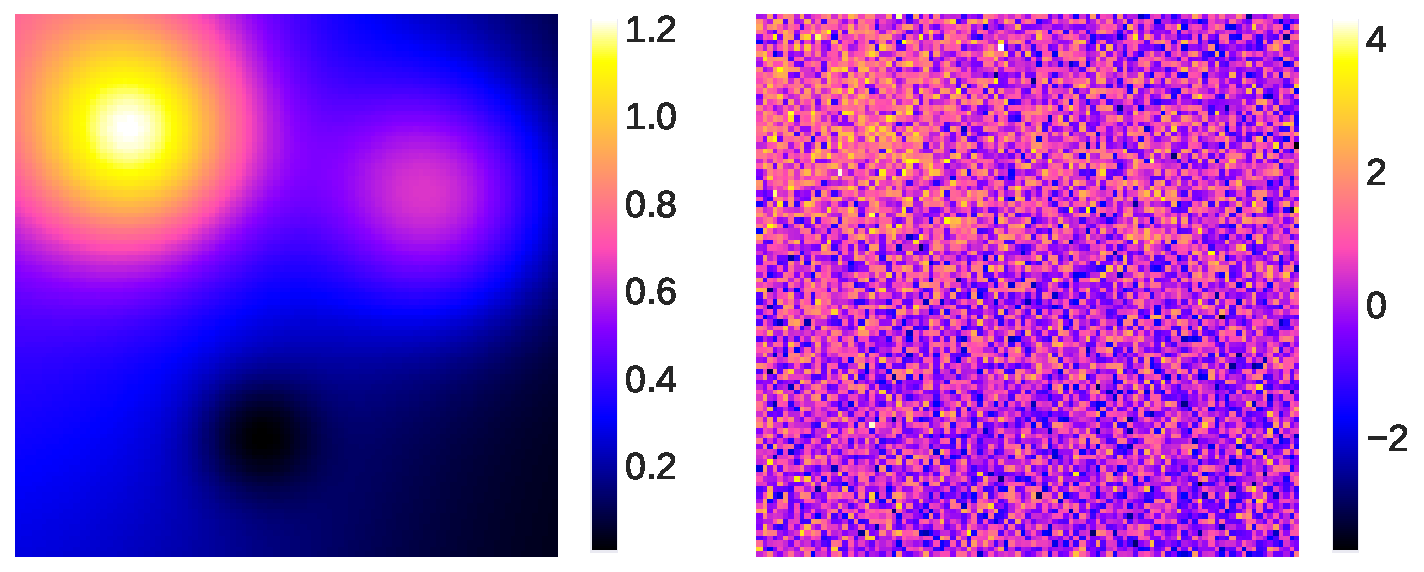
\includegraphics[scale=0.4]{../figs/Franke.pdf}
    \caption{Left: Generic data from Franke's function. Right: Data from Franke's function with added gaussian noise $N(0, 1)$.}
    \label{fig:Franke}
\end{figure}


\subsubsection{Terrain Data}
As a more serious test of our methods, we use elevation data of the south-western part of Norway, gathered from \url{https://earthexplorer.usgs.gov/}, and shown in \cref{fig:Terrain}. The elevation is in units of km, and we use explanatory variables $x,y \in [-1,\, 1]$, just like for the Franke data. The original image is very large, which might present problems with both the runtimes, and exploring the over- and underfitting properties of the different methods. We therefore employ downsampling of the image, usually by 16x16 pixels if nothing else is stated. We average pool over these pixels, resulting in a dataset of $113\cdot 226 = 25538$ datapoints. The downsampled image is shown on the right of \cref{fig:Terrain}.

\begin{figure}[h!]
    \centering
    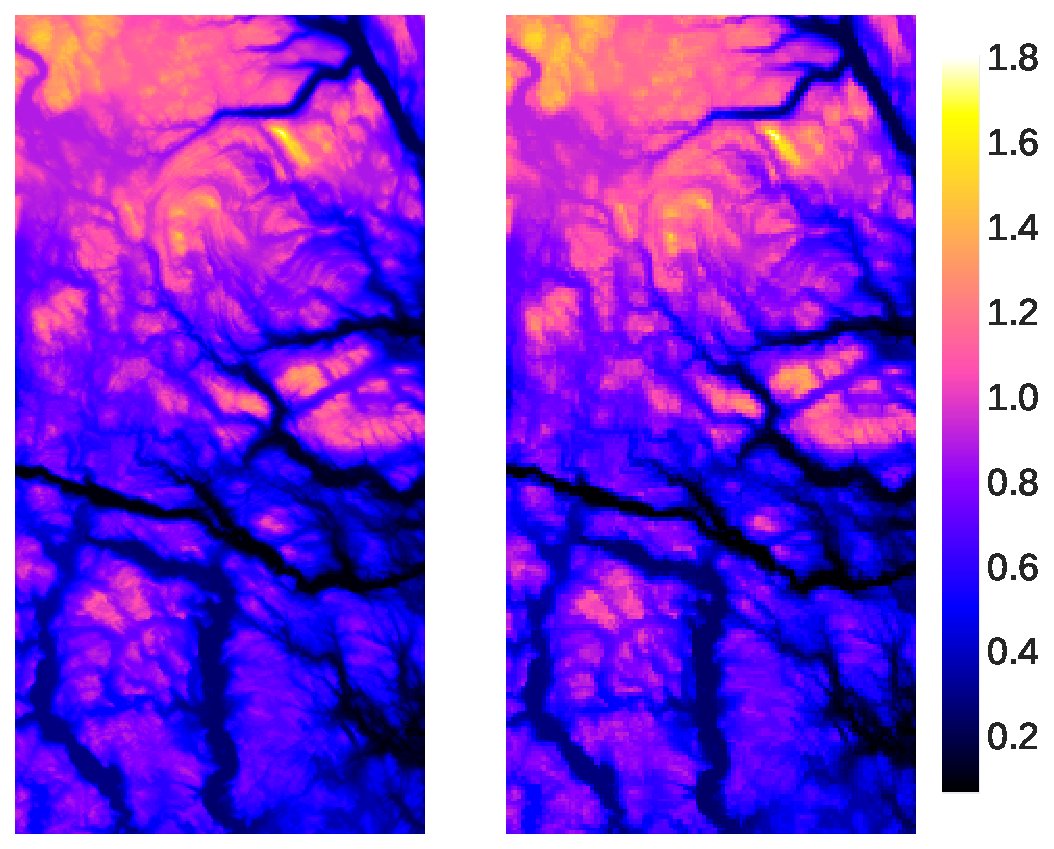
\includegraphics[scale=0.4]{../figs/Terrain.pdf}
    \caption{Left: Elevation map of south-western Norway, 1801x3601 pixels, in units of km. Right: Downsampled version of elevation map on left, 113x226 pixels, with average pooling of 16x16 pixels.}
    \label{fig:Terrain}
\end{figure}

\subsection{Code Structure}
We have utilized a combination of Python files, for back end implementations of classes and function, combined with Jupyter notebooks for running the models and analyzing the data. The analysis is scatter across different notebook files for readability and clarity.

The Regression class in \texttt{regression.py} the back-bone of our whole implementation. This is where we have written methods for every regression method we need, namely OLS, Ridge- and Lasso regression, with and without cross-validation algorithms. We wrote a KFold\_iterator class in the \texttt{KFold\_iterator.py} file, which handles generation of random folds for use of K fold cross validation. Functions for generating generic Franke data can be found in the \texttt{Franke.py} file. All the analysis was implemented across a series of \texttt{.ipynb} files.

While the Ridge and OLS methods have been implemented from scratch, for Lasso, as well as some error metrics and cross validation methods, we use the Python package \texttt{sklearn} from \href{https://scikit-learn.org/stable/documentation.html}{scikit-learn}.



\subsection{Multivariate Polynomial Regression}
We are specifically dealing with polynomial regression with two explanatory variables. This means we have one set of output data, $\vb{f}$, which we attempt to predict as a polynomial of two sets of input data, $\vb{x}$ and $\vb{y}$. 

If we think of $\vb{f}$ as a function of the input variables, $\vb{f} = h(\vb{x}, \vb{y} )$, $\vb{f}$ becomes a surface in two dimensions (or simply a series of heights, since all three are discrete). The polynomial fit will, either way, be a smooth surface in two dimensional space. 

Now, assuming a polynomial of some order $m$, we get a design matrix on the form 
\begin{align}
    \vb{X} = [\b 1\ \ \vb{x} \ \ \vb{y} \b \ \ \vb{x} \vb{y} \ \ ... \ \ \vb{x} \vb{y}^{m-1} \ \ \vb{x}^m \ \ \vb{y}^m]
\end{align}
Where $\vb{X}$ will be a $n\times p$ matrix, where $p = \frac{(m + 1)(m + 2)}{2}$, because of all the crossterms between $\vb{x}$ and $\vb{y}$. Similarly, we have $\vb{\beta}$ as a vector of length $p$.

\subsection{Basic Analysis}
First and foremost, we performed regular OLS regression with a 5th order polynomial and without cross-validation the generated data as described by \cref{eq:franke_w_noise}. This was done mainly as a sanity check, given that we have the luxury of knowing the underlying properties of the data we're trying to fit, making it easy to check if everything yields expected results. An important fact to be aware of when not using any cross validation algorithms is that we are more likely to end up with over fitting our data set. 

This basic analysis consisted of checking the error metrics, namely the MSE and R2 score as described in \cref{subsec:method_errormetrics}. This was done using simply by using the method found in the Scikit-Learn python package: \texttt{sklearn.errormetrics}. We also explored the variance and confidence interval of the $\beta$s, following the logic described in \cref{subsec:confidence_intervals_method}.

Moving on, with confidence in our implementation this far, we performed the same basic analysis on the terrain data. To minimize computational time we downsample the data set as explained in \cref{fig:Terrain}. 

\subsubsection{K Fold Cross Validation}
The next natural step is to implement some form of cross-validation algorithm. We implemented the K fold resampling technique as explained in \cref{subsubsec:kfold_method}. Further on, unless stated otherwise, we will always utilize cross-validation when performing any type of regression, and we will by default use $K=10$.

%Write something about HOW we implemented K-folding? No? Idk im tired man
After implementing K-folding, we tested it by looking at the different error metrics and compare them to the results from regular OLS without K-folding, both on the generated data and the terrain data. We expect that any signs of over fitting should disappear, as we now train and test on different parts of the data sets. 

%To quantify how well a model fits a certain dataset, we will employ K fold validations, and look at the resulting MSE and R2 score values on the testing set. We find K fold validation to be the best and most versatile resampling technique when the quality of a method is to be established and compared to other methods. Especially the ability of K folding to predict on the entire dataset (without cross-contamination between training and testing data) which makes it so versatile. This makes visualizing the predicted model solutions much easier, as the entire input dataset is present in the prediction. The K folding will by default be employed with $K=10$ folds, unless otherwise stated.

\subsubsection{Ridge Regression}
Furthermore, we implemented Ridge regression, with the intent of exploring how this method of regression differs from regular OLS. While there does exist Python packages like Scikit-Learn that performs Ridge regression for you, but as mentioned in \cref{subsec:Ridge}, Ridge regression has an analytical solution for the optimized $\beta$ values, namely \cref{eq:ridge_anal}, which made it possible for to write our own implementation similar to the OLS implementation.  

Adding Ridge regression to our analysis means adding an extra parameter that needs to be optimized for. Choosing the proper $\lambda$ makes a huge difference in how well our model performs. To explore how $\lambda$ affects the error metrics, we simply performed several Ridge regressions, looping over decreasing values of $\lambda$ in the interval $\lambda \in [10^{-8}, 10^3]$ for the Franke data, and $\lambda \in [10^{-8}, 10]$ for the terrain data. We plotted the result of each regression against it's corresponding $\lambda$ value, and compared this to the error metrics obtained from regular OLS. 

\subsubsection{Lasso Regression}
Lasso, while very similar to Ridge, does not have an explicit expression for its optimal $\vb{\beta}$. This means that to explore how $\lambda$ influences our fit, we would have to write an optimization scheme to minimize the cost function, if we wished to write our own implementation. Alas, we did not, so we utilized the Scikit-Learn package \texttt{sklearn.linear\_model.Lasso}. 

As with Ridge, we explored the $\lambda$-dependency of the error metrics by performing several Lasso regressions and plotting the results. Since there's no analytic solution for minimizing the cost function, Lasso has a considerable longer computation time than Ridge, therefore we looked at a smaller interval for the $\lambda$s. For the Franke data, we explored the error metrics for $\lambda \in [10^{-2}, 10^{-8}]$, while for the terrain data we look at the interval $\lambda \in [10^{-2}, 10^{-8}]$. Again, the results of this were compared to the error metrics from OLS. 

\subsubsection{Bias Variance Tradeoff}
\label{subsubsec:Method/Bias_variance_tradeoff}
As discussed in \cref{subsec:Theory/Bias_variance_tradeoff}, overfitting, resulting in high model variance, can be a serious problem for highly complex models. We therefore studied the training and testing MSE of the models for a varying set of complexities. We split the dataset in a training set of $75\%$ and a testing set of $25\%$. The models were thereafter run for polynomial order 0 through 20 for the Franke data, and 0 through 110 for the Terrain data, downsampled by 8x8. A $\lambda = 10^{-4}$ used for Ridge and Lasso. We also downsampled the terrain data to 32x32, from polynomial order 0 through 35, to see how a reduction in dataset size would impact the overfitting.

We also studied the numerical stability of the model. If the matrix $\vb{A}= \vb{X^T}\vb{X}$ is ill-conditioned, we might observe unstable or supressed results. The test and train MSE of Ridge and OLS was run for polynomial orders 0 through 65, for a shifted set of explanatory variables, $x,y \in [0,\, 2]$. The condition number of the matrix $\vb{A}$ for OLS and Ridge for $\lambda = 10^{-2}$ and $\lambda = 10^{-6}$ was plotted against polynomial orders 0 through 60. This was repeated for the shifted explanatory variables.

%\subsubsection{Something about bootstrap?}
%too many subs?
\subsubsection{Calculating the Bias and Variance}
While the method described in the former section allowes us to see the effect of over- and underfitting, it is also of interest to study the actual values of bias and variance. We can separate the contributions to the MSE into bias and variance as discussed in \cref{subsec:Theory/Bias_variance_tradeoff}, but we need to some way to calculate the expectation value of our fit given slightly different training sets. To do this, we implemented the Boostrap method from \cref{subsubsec:Theory/Boostrap}. The data is split in a training set of $75\%$ and a testing set of $25\%$. The bootstrap is then performed on the training data only, testing on the same testing set each time. After $k$ boostraps we are left with multiple slightly different fits, which we used to calculate the quantities involved in the bias and variance terms of the MSE. In this way we usually can't quantify the irreducible error $\sigma^2$, as this is generally unknown. So the sum of the bias and the variance should be less than the actual MSE.

The bootstrap was performed with OLS, Ridge and Lasso, on both Franke and Terrain data. For Ridge and Lasso, we used $\lambda=10^{-4}$. For the Franke data, we performed the bootstrap for polynomial orders from 1 through 20, and 1 through 28 for the terrain data. 



\subsection{Numerical Limitations}
\label{subsubsec: numerical_limitations_method}
There might be limitations posed upon the complexity of our model by our numerical accuracy. Our design matrix will hold polynomials of increasing order, up until some last column of order $\b x^m$. This column might differ hugely in magnitude to the first column, which is of order $1$. The decision of how to scale the explanatory variables $\b x$ and $\b y$ might have a lot of impact on the numerical stability of the design matrix. We have chosen to space our explanatory variables in $[-1, 1]$ to limit such effects.

If an interval for $\b x$ and $\b y$ smaller than this is chosen, the entire columns will be largely suppressed. Say an interval of $[-0.5, 0.5]$ was chosen, it would have its largest value suppressed to $0.5^m$. Around $m=50$, it would lose approximately all its significant digits in an arithmetic operation with $1$, because $0.5^{50} \approx 10^{-15}$, approaching double float precision compared to $1$. The columns of polynomial order $50$ or higher in the design matrix would for all intents and purposes be 0. Choosing an interval exceeding 1, like $[-2, 2]$, might be even worse, as it would render the \textit{first} columns practically zero instead of the last, ruining the lower order polynomials.

Choosing an interval $[-1, 1]$ in no way solves the problem, as much of the column will be suppressed to zero at higher orders, but neither does it entirely blow up or down, and seemed like the best choice. For OLS especially, the suppressed later columns might lead to a singular or extremely ill-conditioned matrix. Pseudo-invertation, as discussed in \cref{subsec:singularity} will be employed to mitigate this problem.


% ██████╗ ███████╗███████╗██╗   ██╗██╗  ████████╗███████╗
% ██╔══██╗██╔════╝██╔════╝██║   ██║██║  ╚══██╔══╝██╔════╝
% ██████╔╝█████╗  ███████╗██║   ██║██║     ██║   ███████╗
% ██╔══██╗██╔══╝  ╚════██║██║   ██║██║     ██║   ╚════██║
% ██║  ██║███████╗███████║╚██████╔╝███████╗██║   ███████║
% ╚═╝  ╚═╝╚══════╝╚══════╝ ╚═════╝ ╚══════╝╚═╝   ╚══════╝
\section{Results}
\subsection{Ordinary Least Squares analysis}
\subsubsection{Franke Data Without Cross-Validation}
In \cref{tab:Franke_metrics_no_kfold} we see the results of performing an ordinary polynomial regression on \cref{eq:franke_w_noise} using a polynomial of order $5$. Since we have the luxury of working with a data set where we know what the underlying function should look like, we compare our fit both to the noisy data, and the clean Franke function. First and foremost, we notice that the MSE when compared to the noisy data is less than $1$. As we have full control of the generated noise in our data set, and we have set this noise to be Gaussian with a standard deviation $\sigma=1$, we know that the MSE should not go lower than $1$. Thus, what we observe here seems to be a classic case of over-fitting, which is not surprising considering we have not yet implemented any type of resampling or cross-validation, meaning we are training and testing on the same data.

Aside from that, we see that when comparing to the underlying function, the MSE score is pretty close to $0$, and the R2 score is not that far from $1$.

\begin{table}
\centering
\begin{tabular}{l|l|l|}
\cline{2-3}
                                              & \textbf{MSE} & \textbf{R2} \\ \hline
\multicolumn{1}{|l|}{\textbf{Franke + noise}} & 0.997        & 0.047       \\ \hline
\multicolumn{1}{|l|}{\textbf{Noiseless}}      & 0.004        & 0.843       \\ \hline
\end{tabular}
\caption{Table showing the MSE- and R2 score when performing ordinary polynomial regression on the generated noisy data (\cref{eq:franke_w_noise}) without any resampling techniques. The upper row contains the errors calculated with respect to the noisy data, while the lower row shows the errors with respect to the underlying Franke function with no added noise.}
\label{tab:Franke_metrics_no_kfold}
\end{table}




\subsubsection{Franke Data with Cross-Validation}
In \cref{fig:franke_ols}, we see the result of fitting \cref{eq:franke_w_noise} with a 5th order polynomial using OLS regression and the K-fold cross-validation algorithm compared with the underlying noiseless Franke function. Here we observe that the MSE on the testing data is no longer lower than $1$ when compared to the noisy data, because we are no longer training on our test data, meaning we cant over-fit on it.

\begin{table}[h!]
\centering
\begin{tabular}{l|l|l|}
\cline{2-3}
                                              & \textbf{MSE} & \textbf{R2} \\ \hline
\multicolumn{1}{|l|}{\textbf{Franke + noise}} & 1.001        & 0.047       \\ \hline
\multicolumn{1}{|l|}{\textbf{Noiseless}}      & 0.004        & 0.820       \\ \hline
\end{tabular}
\caption{Table showing the MSE- and R2 score when performing OLS regression with K-folding. The upper row shows the error metrics when compared with the noisy data, while the lower row contains the error when comparing to the clean Franke function.}
\label{tab:Franke_metrics}
\end{table}

A visual comparison of the underlying Franke function and our polynomial fit can be seen in \cref{fig:franke_ols}. While stating that \textit{"they clearly look alike"} is not the most scientific way of deciding whether a method yields sufficient results or not, they \textbf{do} clearly look similar! 

\begin{figure}[h!]
    \centering
    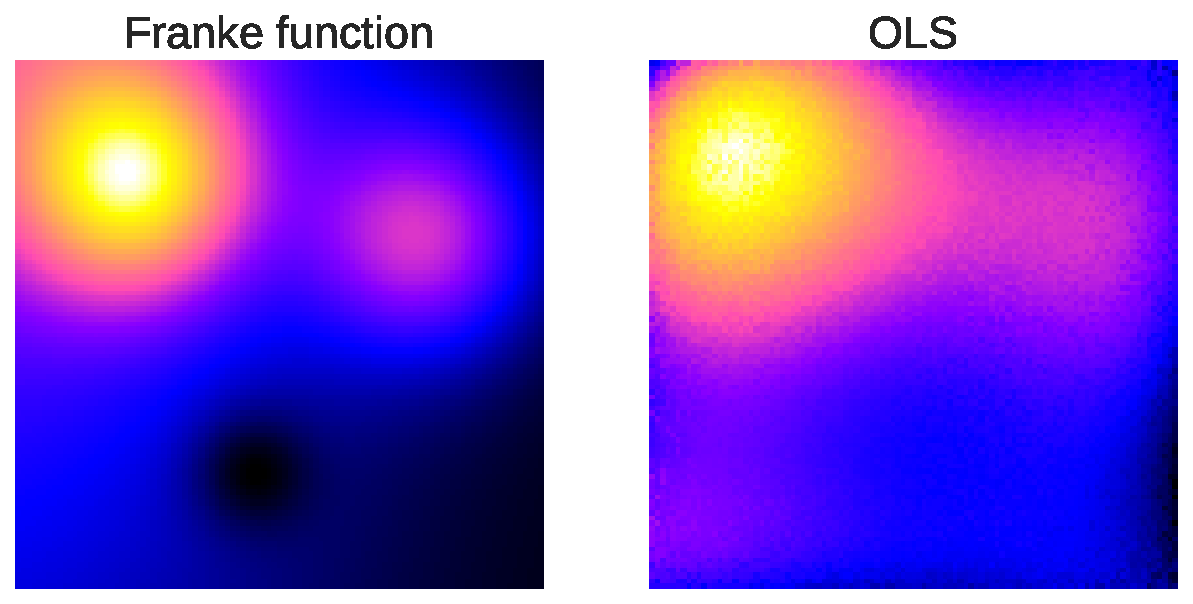
\includegraphics[scale=0.4]{../figs/franke_vs_ols.pdf}
    \caption{Figures comparing the Franke function without noise (left) and the prediction made using OLS with a 5th order polynomial and K-folding with K=10 (right).}
    \label{fig:franke_ols}
\end{figure}

\subsubsection{Terrain Data}
In \cref{tab:error_metrics_terrain_data_ols} we see the MSE and R2 score when trying to fit the terrain data to a polynomial of order 5 using regular OLS and k-folding with k=10. Given the low R2-score we can conclude that a 5th order polynomial might not be the best fit for this data-set. Intuitively, this makes sense, as a terrain will be made up of a high number of nooks and crannies which is not possible to represent with a polynomial with such a low order.
\begin{table}[h!]
\centering
\begin{tabular}{l|l|l|}
\cline{2-3}
                                            & \textbf{MSE} & \textbf{R2} \\ \hline
\multicolumn{1}{|l|}{\textbf{Terrain data}} & 0.042        & 0.456       \\ \hline
\end{tabular}
\caption{Table showing the error metrics when fitting the terrain data using OLS regression with a polynomial of order 5 and k-folding with K=10.}
\label{tab:error_metrics_terrain_data_ols}
\end{table}

The quality of the fit can also be seen in \cref{fig:terrain_ols}. Here we see that, while a 5th order polynomial does preserve the overall shape of the data, it does not do a good job at replicating the finer details. How the error metrics behave for a model with higher complexity is explored more closely later on. 

\begin{figure}[h!]
    \centering
    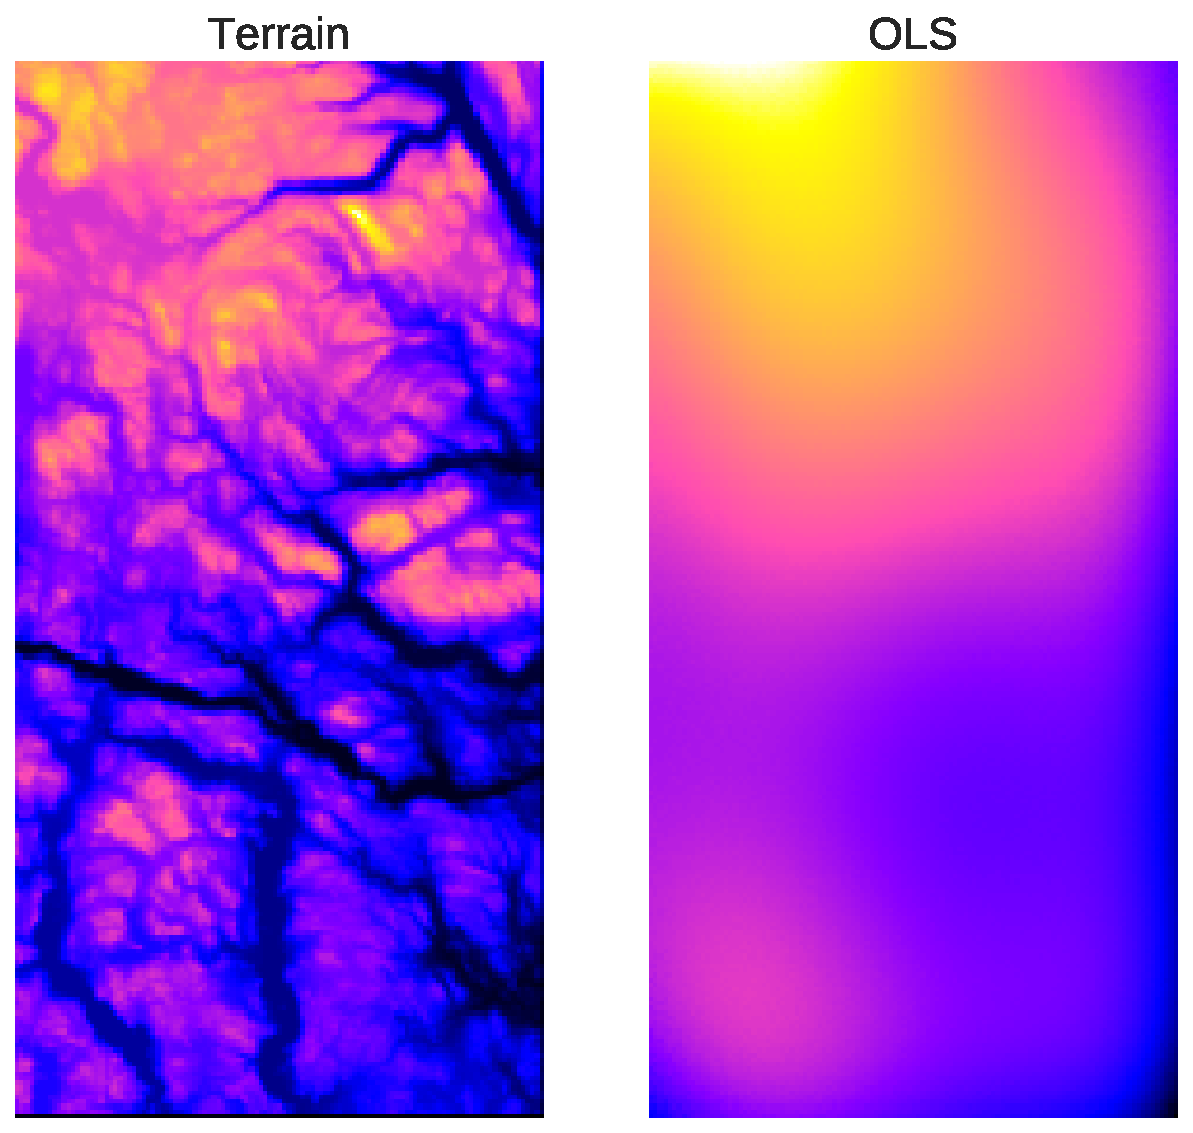
\includegraphics[scale=0.4]{../figs/terrain_vs_ols.pdf}
    \caption{Figures comparing the terrain data (left) and the prediction made using OLS with a 5th order polynomial, and K-folding  with K=10 (right).}
    \label{fig:terrain_ols}
\end{figure}

\subsection{Confidence Intervals}
In \cref{fig:CI_Franke} we see the predicted values of the $\beta$ coefficients of the OLS model on Franke data, with 95\% confidence intervals. The variance of each $\beta$ is also plotted below. Since our explanatory variables are nothing but different polynomial orders of the x and y axis, the coefficients doesn't have very obvious interpretations, and neither does their confidence intervals. Either way, the ranges seem neither very large nor very small. We note that $\beta_0$, the intercept, has a significantly smaller variance than the other coefficients.

In \cref{fig:CI_Terrain} the same values are plotted for the OLS fit on Terrain data, downsampled by 32x32. Here, the confidence intervals and variances are, relatively, substantially smaller than in the Franke case. The variances are on the scale ~0.1 the typical size of the $\beta$s, while this ratio is closer to ~0.5 for the Franke data. This is very stange, as OLS obviously made a worse fit on the Terrain data than it did the Franke data, and we would expect the opposite result. We have no good explanation for this, but expect it to be some error.

Another odd observation is the relative size of the $\beta$ variances between Franke and Terrain data. Looking at the two figures, we observe that they have the exact same shape. The ratio of variance between the coefficients is the same, even though their values differ. Looking back at the definition of the variance in \cref{subsec:confidence_intervals_method}, this result shouldn't be surprising at all, since the variance is nothing but a scalar quantity multiplied by the diagonal elements of $\vb{X^T}X$. Since we defined the x and y axis to be linearly spaced in the same interval, $[-1,\, 1]$, for both Franke and the Terrain data, their design matrices, and therefore also $\vb{X^T}X$, are identical. This means the ratio between the variances of the $\beta$s are equal by design. We found this as rather odd. Our intuition tells us the data we are trying to fit, and thereby what the final fit becomes, should have some impact in the confidence of the coefficients. Either our inuition is wrong, or we overlooked something in the calculation of the confidence intervals. The data \textit{does} come into play in the scalar quantity we multiply by, but this scales all the variances equally, meaning the data doesn't impact the ratio between the variances.

\begin{figure}[h!]
    \centering
    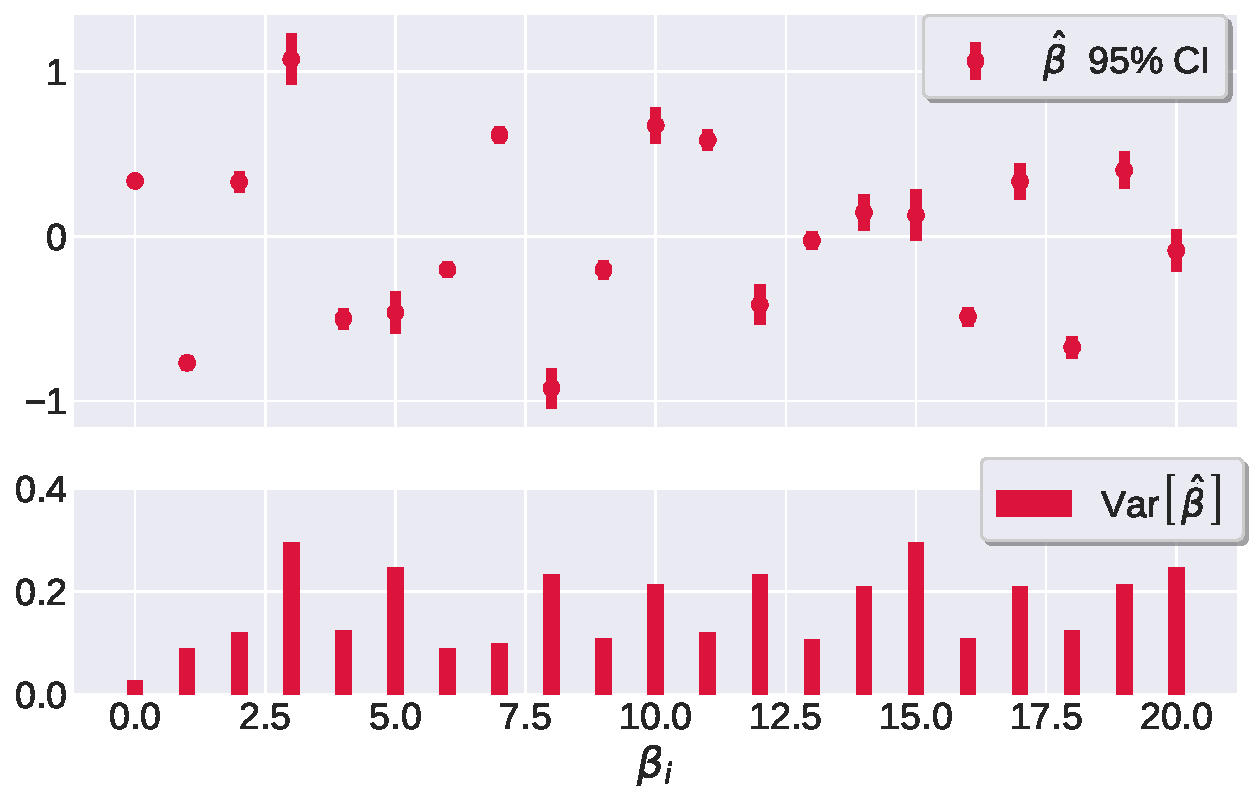
\includegraphics[scale=0.4]{../figs/CI_Franke.pdf}
    \caption{Regression fit of 5th order polynomial on Franke data, using OLS with K-folding. Top: Predicted $\beta$s with 95\% confidence intervals. Bottom: Variance of predicted $\beta$s.}
    \label{fig:CI_Franke}
\end{figure}

\begin{figure}[h!]
    \centering
    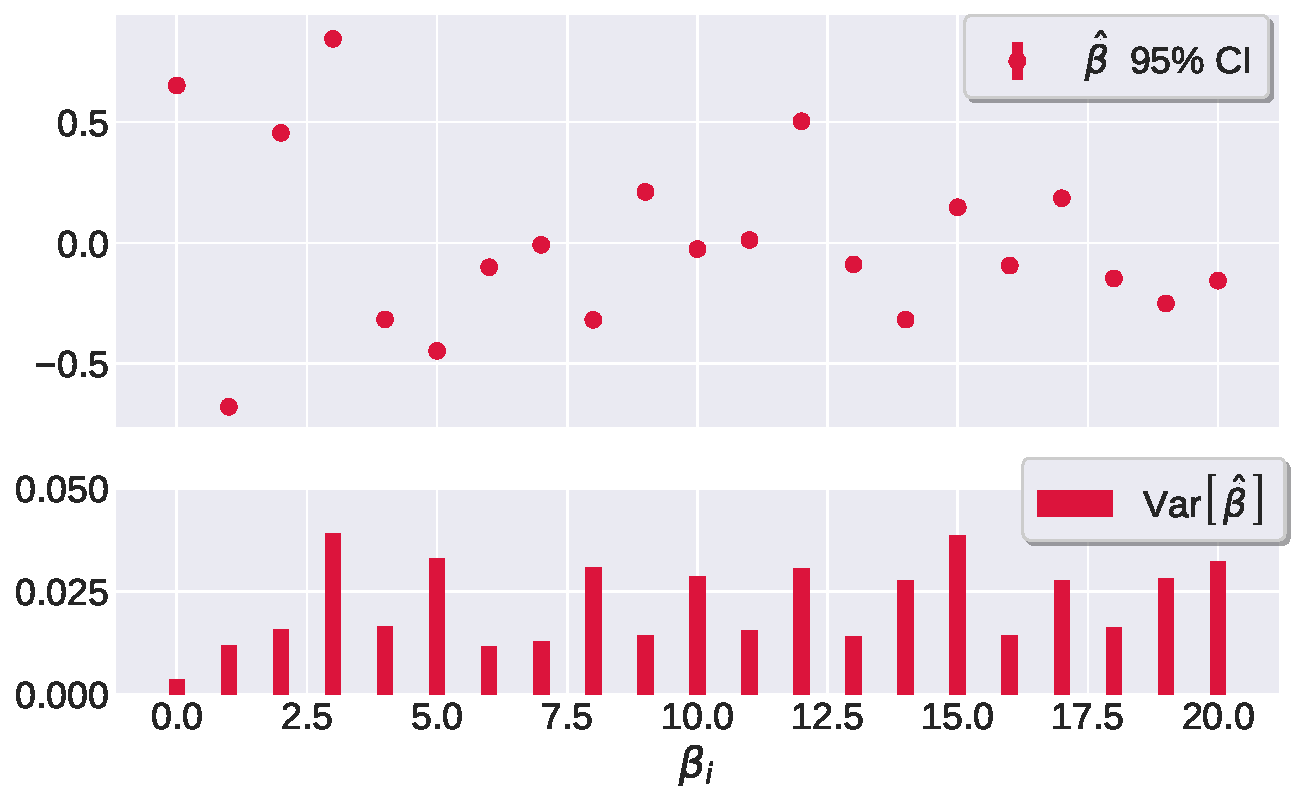
\includegraphics[scale=0.4]{../figs/CI_Terrain.pdf}
    \caption{Regression fit of 5th order polynomial on Terrain data, using OLS with K-folding. Top: Predicted $\beta$s with 95\% confidence intervals. Bottom: Variance of predicted $\beta$s.}
    \label{fig:CI_Terrain}
\end{figure}



\subsection{Ridge, Lasso and $\lambda$-dependence}
\subsubsection{Franke Data}
In \cref{fig:lambda_ridge_franke} and \cref{fig:lambda_lasso_franke} we explore how the MSE changes as a function of the hyperparameter $\lambda$ when fitting the data using Ridge regression and Lasso regression respectively. 

First and foremost, we see that when using Lasso regression, we need a significantly lower value for $\lambda$ when compared to Ridge regression if we wish to reach the same accuracy as with regular OLS. For Ridge, we see that for $\lambda < 10^1$, we get approximately the same precision as with regular OLS, while with Lasso we need a $\lambda < 10^{-4}$ to reach sufficient accuracy. 
\begin{figure}[h!]
    \centering
    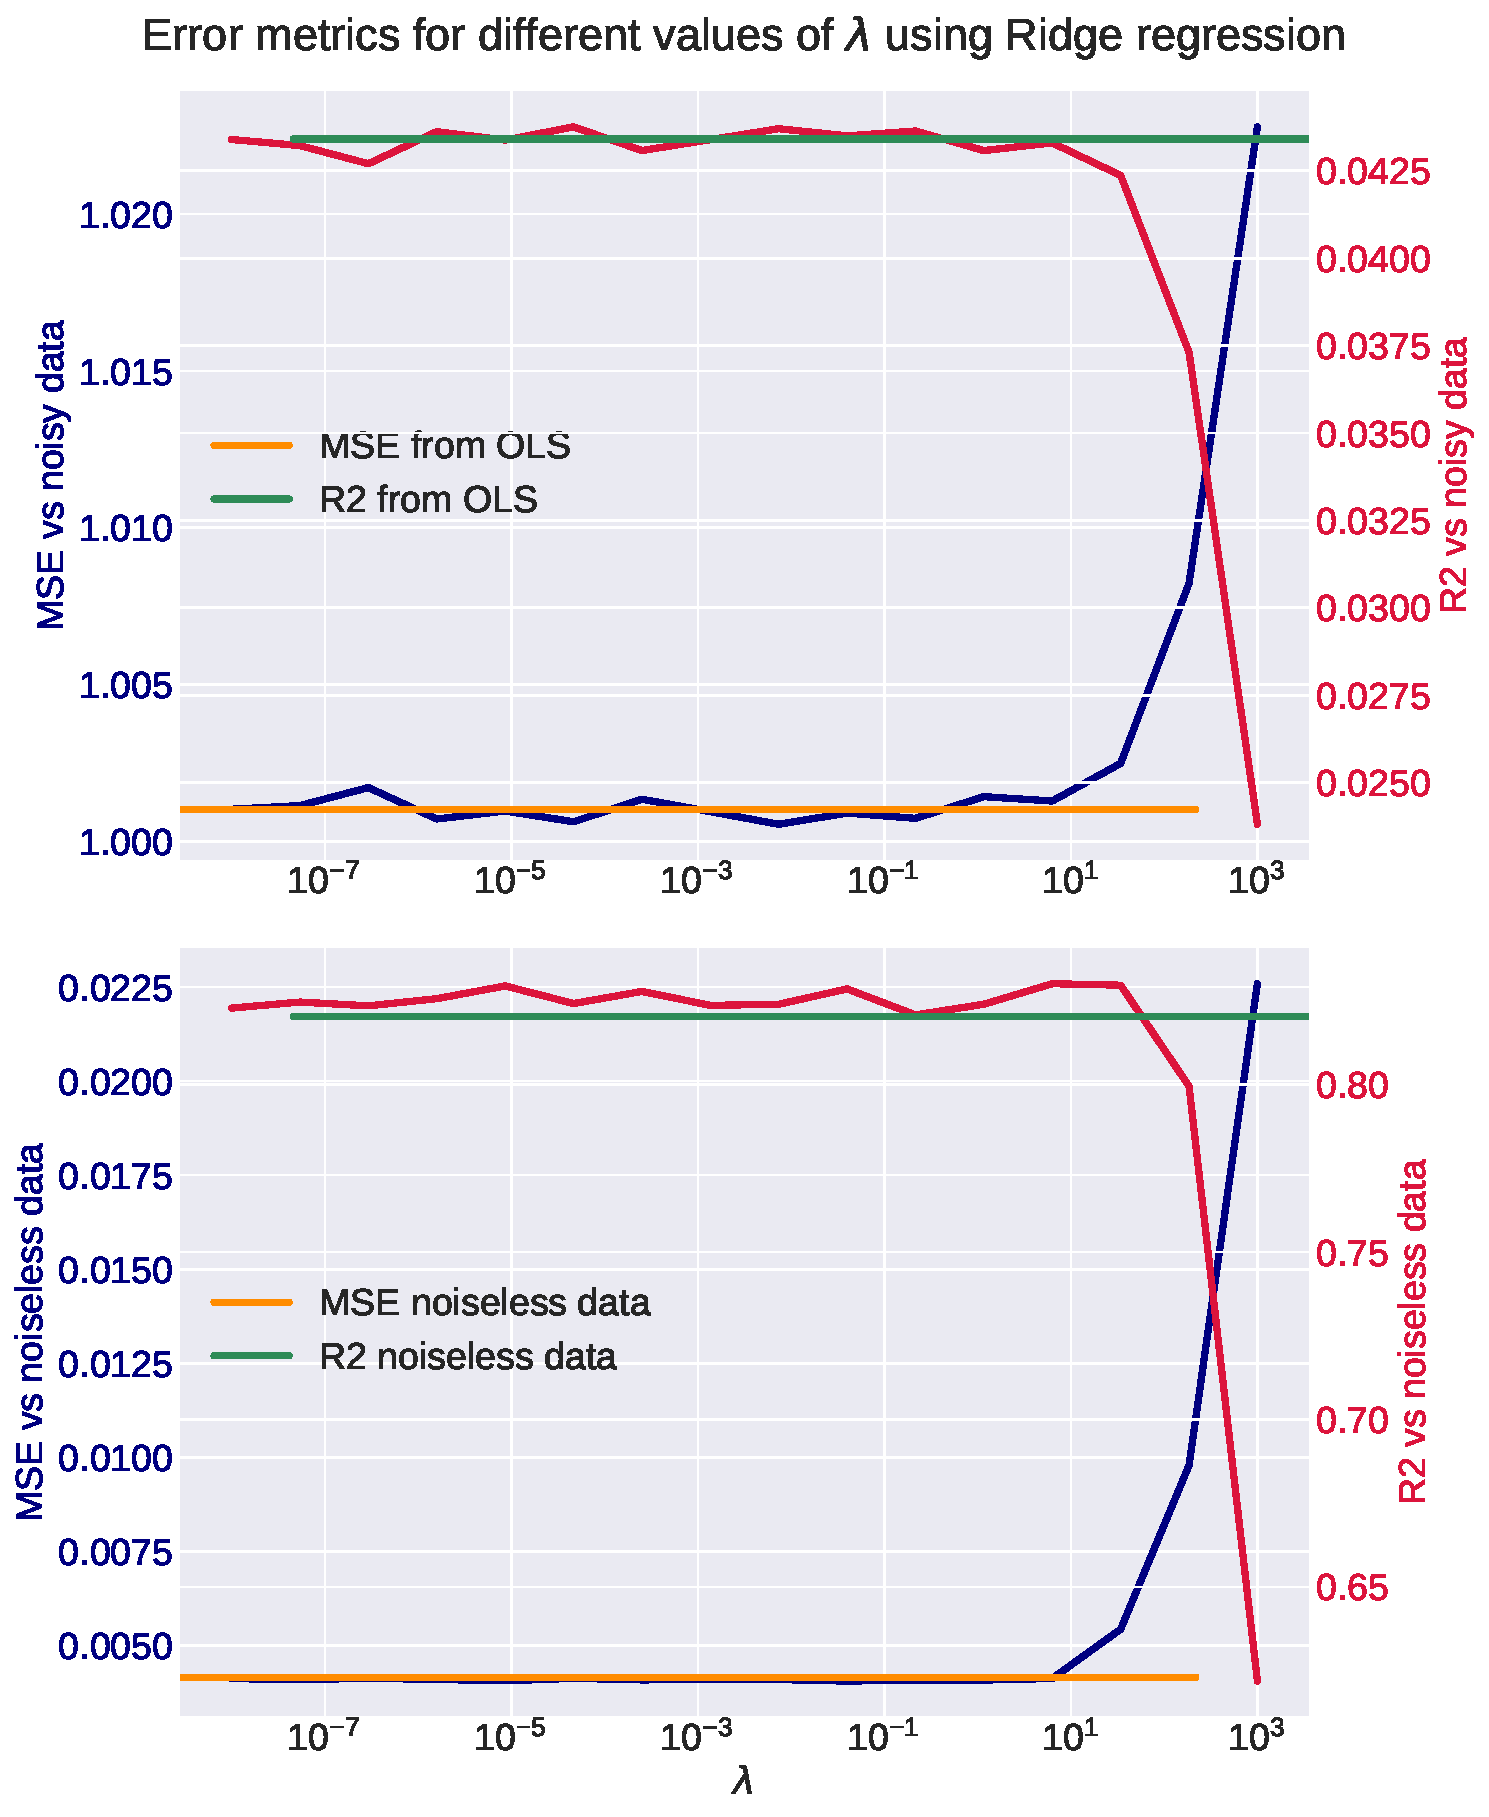
\includegraphics[scale=0.4]{../figs/errormetrics_lambda_ridge_franke.pdf}
    \caption{Plots showing how the MSE- and R2 score behaves for increasing values of $\lambda$. The upper plot illustrates these metrics when comparing the predicted fit from Ridge regression to the Franke function with added noise. The lower plot shows the behavior of these metrics when comparing the fit to the noiseless Franke function. The lines represent the MSE and R2-score acquired from OLS regression.}
    \label{fig:lambda_ridge_franke}
\end{figure}

\begin{figure}[h!]
    \centering
    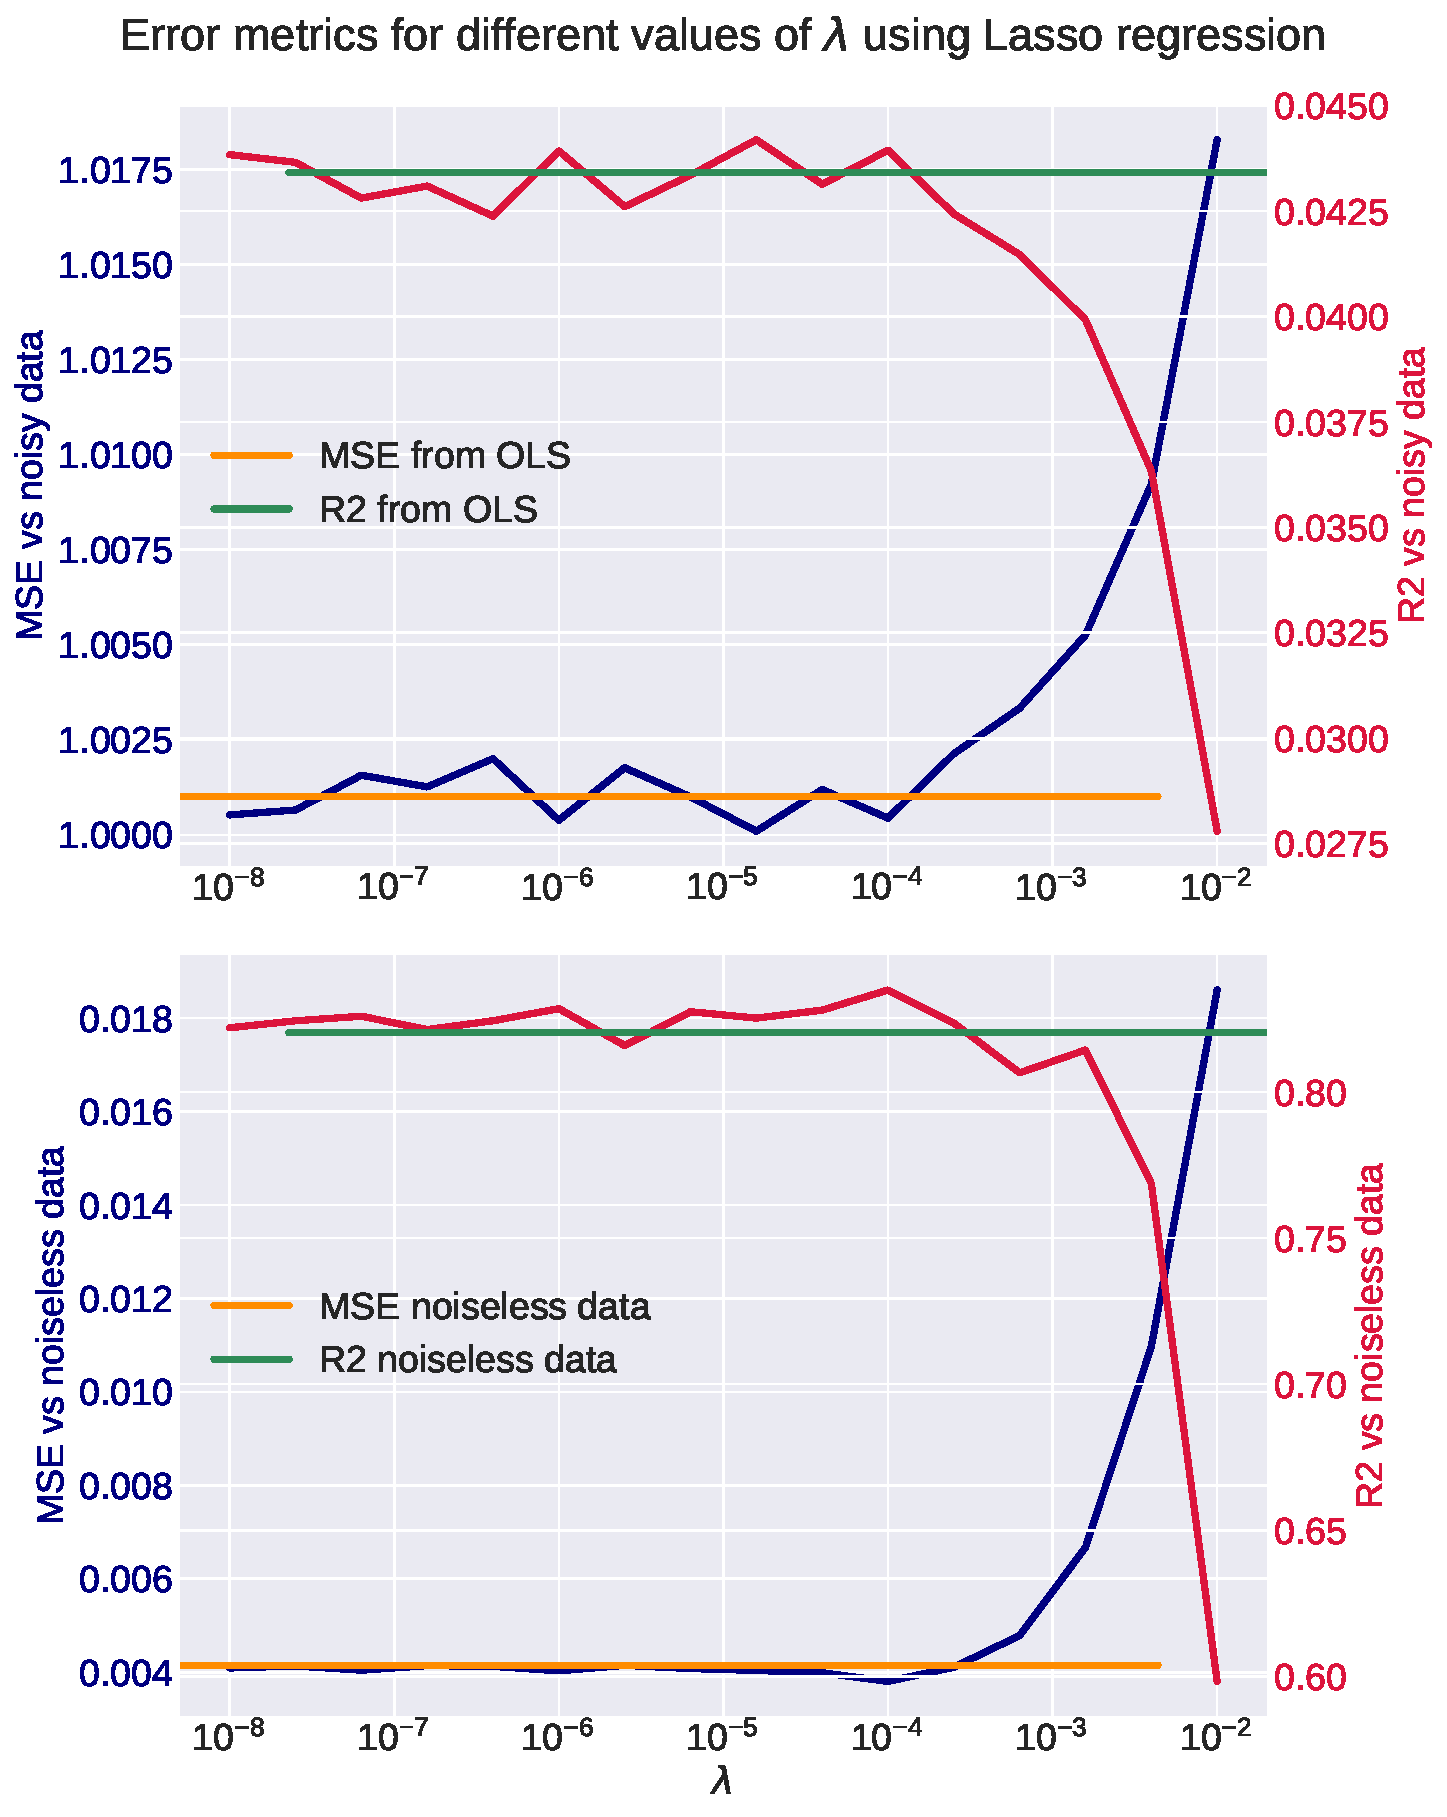
\includegraphics[scale=0.4]{../figs/errormetrics_lambda_lasso_franke.pdf}
    \caption{Plots showing how the MSE- and R2 score behaves for increasing values of $\lambda$. The upper plot illustrates these metrics when comparing the predicted fit from Lasso regression to the Franke function with added noise. The lower plot shows the behavior of these metrics when comparing the fit to the noiseless Franke function. The lines represent the MSE and R2-score acquired from OLS regression.}
    \label{fig:lambda_lasso_franke}
\end{figure}

\subsubsection{Terrain Data}
As with the generated Franke data, we wish to explore how the error metrics behave as a function of $\lambda$ for both Ridge and Lasso regression on the terrain data set. The results of this can be seen in \cref{fig:lambda_ridge_terrain} and \cref{fig:lambda_lasso_terrain}. Unexpectedly, we see the same trend here, where we need a much lower value for $\lambda$ to reach sufficient accuracy with Lasso compared to Ridge. When using Ridge regression we reach OLS error metrics when $\lambda < 10$, while Lasso doesnt converge until $\lambda < 10^{-7}$.
\begin{figure}[h!]
    \centering
    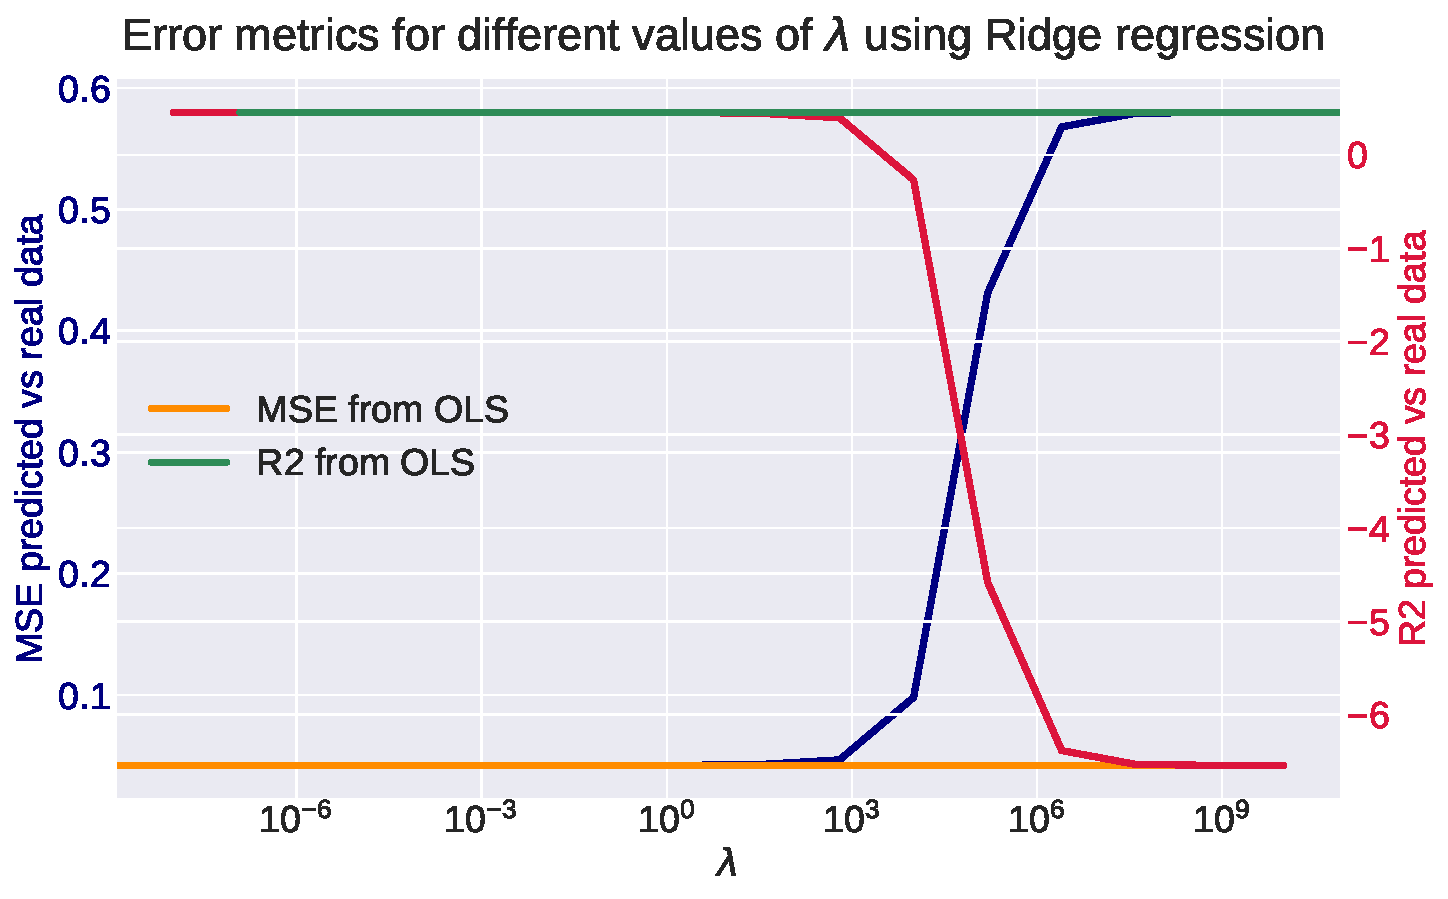
\includegraphics[scale=0.4]{../figs/errormetrics_lambda_ridge_terrain.pdf}
    \caption{Plot showing how the MSE and R2-score behaves for different values of $\lambda$ when doing Ridge regression on the terrain data. The lines represent the error metrics obtained from regular OLS.}
    \label{fig:lambda_ridge_terrain}
\end{figure}

\begin{figure}[h!]
    \centering
    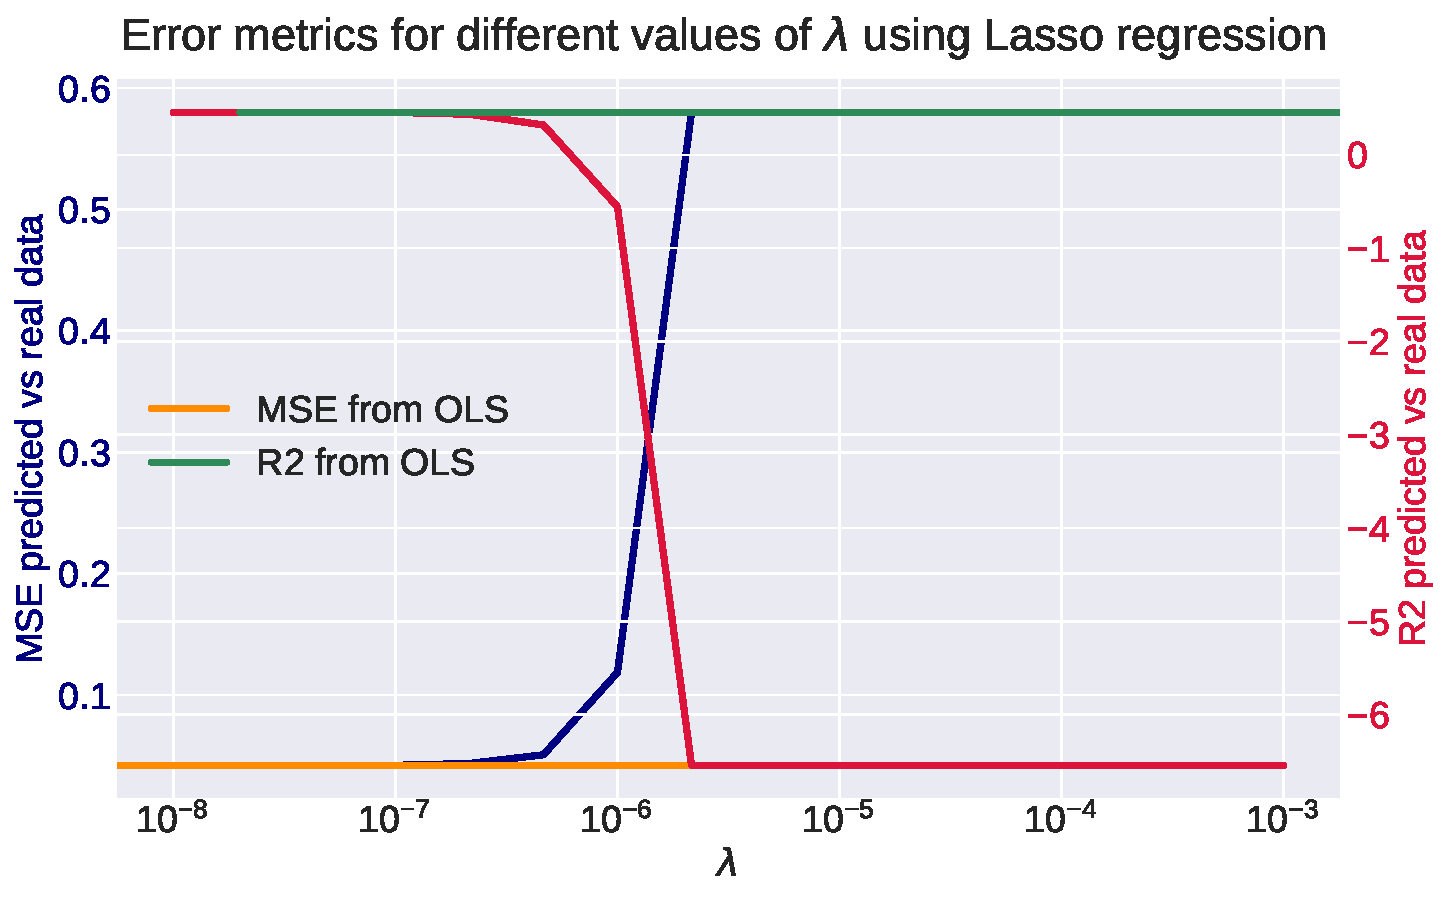
\includegraphics[scale=0.4]{../figs/errormetrics_lambda_lasso_terrain.pdf}
    \caption{Plot showing how the MSE and R2-score behaves for different values of $\lambda$ when doing Lasso regression on the terrain data. The lines represent the error metrics obtained from regular OLS.}
    \label{fig:lambda_lasso_terrain}
\end{figure}

\subsection{Bias Variance Tradeoff}
\subsubsection{Franke Data}
As discussed in section \cref{subsec:Theory/Bias_variance_tradeoff}, a high complexity model might lead to overfitting to the training data. In our case, complexity corresponds to the polynomial order of our model. In \cref{fig:bias_var_franke}, the train and test MSE of Franke data is shown, for all three regression methods. Clear signs of overfitting (high model variance) is shown for OLS at higher polynomial orders. This manifests itself as an increase in testing error, while the training error still decreases. As discussed in \cref{subsec:Theory/Bias_variance_tradeoff}, this is due to the model finding false trends in the training data, that doesn't actually exist in the underlying model. A high complexity model will fit to these trends, which won't exist in the testing set, and therefore lead to an increased error.

The trend is also visible in Ridge regression, but with a substantially lower slope in the error, indicating a stronger resistance to overfitting. Lasso regression is virtually immune to overfitting at higher complexities, having almost no slope at all. All models seem to reach a testing error minimum around polyomial order 5, increasing for higher orders, but at vastly different rates.

It's however still interesting to note that under an ideal complexity (e.g. poly order 5), OLS outperforms the two other models, with a slightly lower testing error.

Another interesting observation is that the testing error on OLS and Ridge fall below 1 around polynomial order 7.5. This itself is an indication of overfitting, as our data is generated with $\mathrm{MSE} = 1$ by design. The noiseless Franke's function, the function we're trying to reproduce, has an MSE of 1 compared to our data. Gaining an MSE lower than this indicates that we're finding trends that doesn't exist in the underlying model. Lasso interestingly converges on a training error of exactly 1.

\begin{figure}[h!]
    \centering
    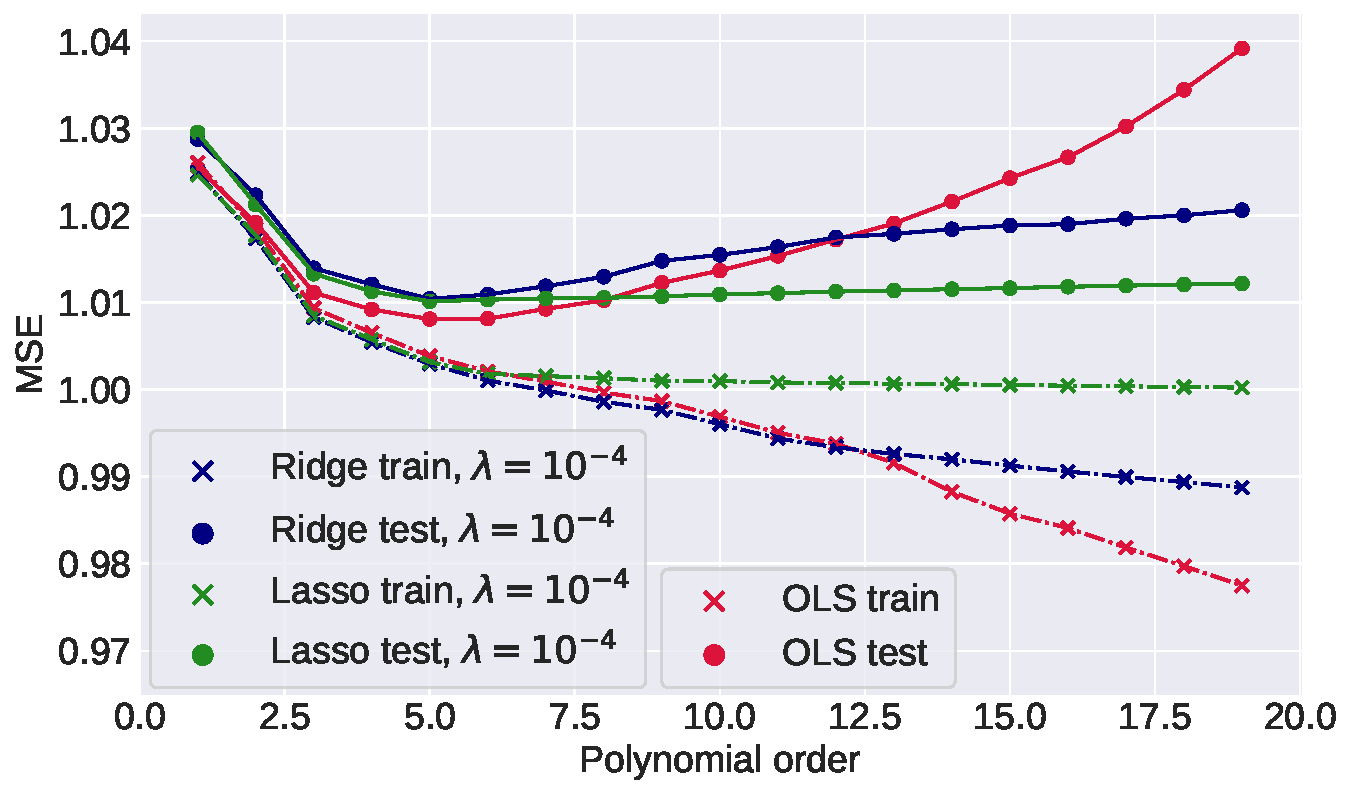
\includegraphics[scale=0.4]{../figs/Franke_OLS_Ridge_polyorders.pdf}
    \caption{Plot showing the MSE of testing and training data for OLS, Ridge, and Lasso as function of polynomial order, using K fold validation on the Franke data. $\lambda = 10^{-4}$ was used for Ridge and Lasso. We see that Lasso keeps a much more stable MSE for increased complexity, while the MSE on the OLS testing data rapidly diverges, indicating an overfitted model. Ridge falls somewhere in between.}
    \label{fig:bias_var_franke}
\end{figure}


\subsubsection{Franke Data Bootstrap}
Using the boostrap method as discussed in \cref{subsubsec:Method/Bias_variance_tradeoff} we are able to calculate the separate components in the MSE to get a deeper insight into the evolution with polynomial order. Here we include only the result from OLS, while similar results for Ridge and Lasso may be found in appendix \ref{asec:Bias_Var_results}. In \cref{fig:Boostrap_franke_ols} are the results for the Franke data set. As expected we see how the bias is high for low complexity, as a result of underfitting. For increasing complexity the variance start increasing and the bias drops, which leads to a minimum in the MSE at polynomial order $\sim 4,5$. At higher complexity the model start overfitting, which is evident in the increase of the variance leading to an increase in the MSE. We note however that we also get a similar increase in the bias for higher complexity. This is not expected and the reason is not understood. Also, as in this case the irreducible error is known we have subtracted it from the MSE and the bias.

\begin{figure}[h!]
    \centering
    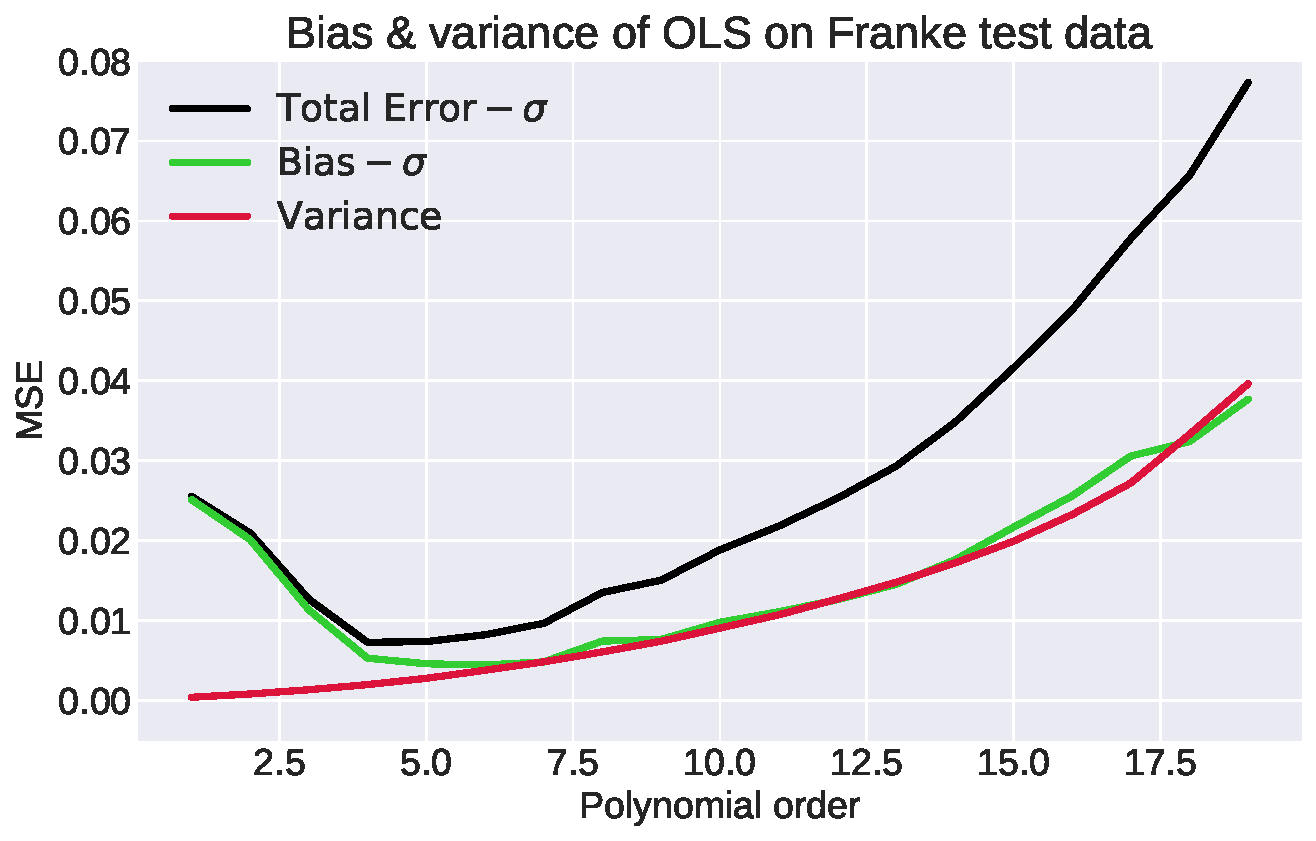
\includegraphics[scale=0.4]{../figs/BV_bootstrap_Franke_OLS.pdf}
    \caption{Plot showing the bias variance tradeoff as a function of polynomial order on the Franke test set. Here we can clearly see how the underfitting at low complexity is evident in the bias. While for higher complexity the model start overfitting and the variance of the model increase. However, we note that the bias also start increasing along with the variance for higher complexity which is unexpected. The reason for this is still unknown.}
    \label{fig:Boostrap_franke_ols}
\end{figure}

\subsubsection{Terrain Data}
Looking at the real terrain data, the picture becomes a bit more complicated due to a number of factors, mostly related to the fact that this dataset contains considerably more points, leading to numerical limitations on the complexity.

\Cref{fig:Terrain_8x8_poly100} shows the train and test error of OLS and Ridge on the terrain data downsampled by 8x8. Here we are, up to seemingly arbitrary complexity, unable to provoke overfitting on either methods, which both remain constant at higher orders. Our theory is that we have reached a level of complexity which is too numerically unstable and ill-conditions to give reliable results. Even if there in theory was a complexity which provoked overfitting in the methods, we might be unable to see them due to suppression of the higher order terms in the design matrix, as discussed in \cref{subsubsec: numerical_limitations_method}. After a certain order, the columns of the design matrix become virtually zero-filled, compared to earlier columns. Increasing the complexity therefore has no effect on the solution.

Another observation is that OLS seems to substantially outperform Ridge in this scenario. This is probably due to the fact that the small $\lambda$ added to the Hessian matrix ends up disturbing higher order terms, which are themselves very small. This is of course some of the idea behind Ridge, but in this scenario where overfitting isn't an issue, it actually ends up huring the predictions.



\begin{figure}[h!]
    \centering
    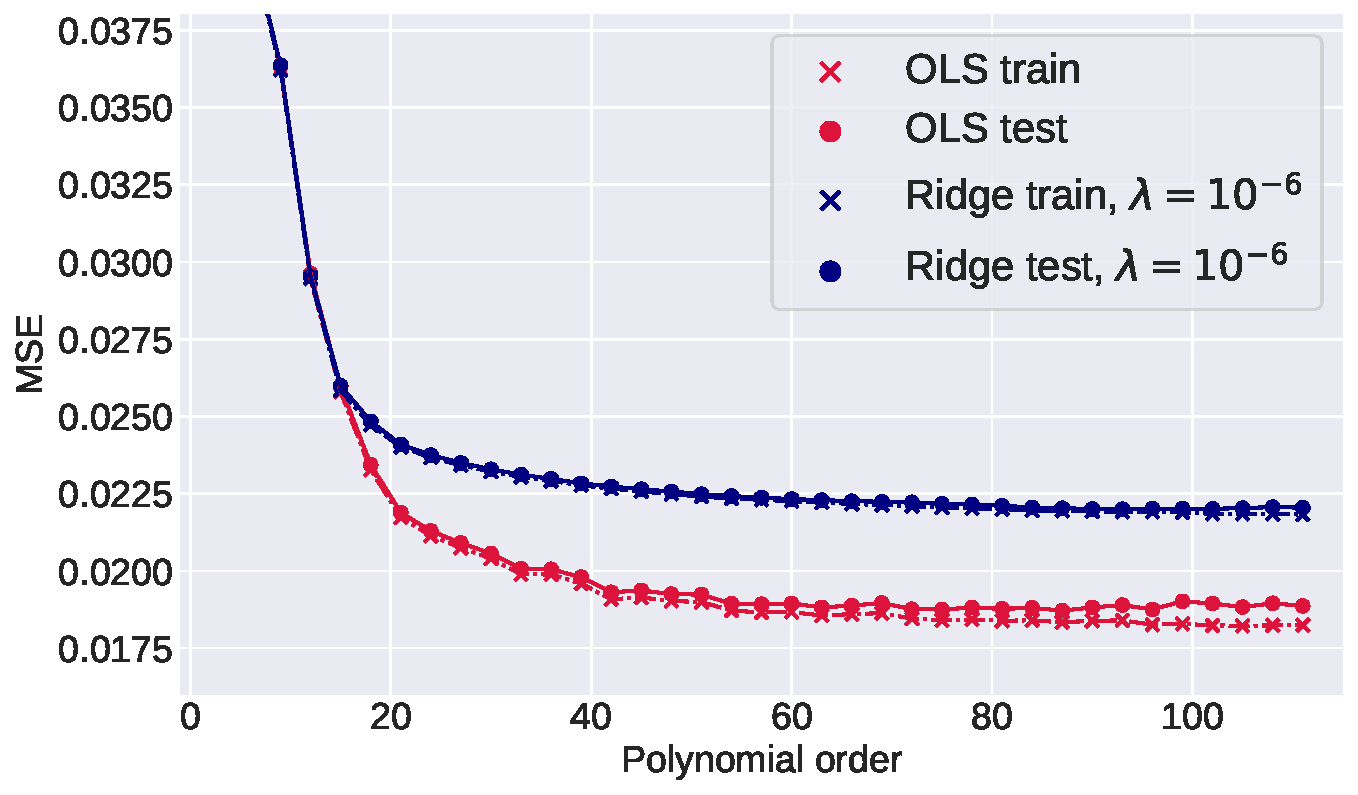
\includegraphics[scale=0.4]{../figs/OLS_Ridge_8sample_poly110.pdf}
    \caption{Plot showing the MSE of testing and training data for OLS and Ridge as function of polynomial order, using K fold validation on Terrain data, downsampled by 8x8. There is no sign of overfitting on either model, even up to very high orders, which might indicate that overfitting occurs at a level of complexity we can't numerically represent, due to suppression of high order terms in the design matrix.}
    \label{fig:Terrain_8x8_poly100}
\end{figure}



Like discussed in \cref{subsubsec: numerical_limitations_method}, this would blow up reversely if our explanatory variables were in a range exceeding one. In \cref{fig:0to2divergence}, we have done exactly this, letting them be in the range $[0,\, 2]$. Analytically, this should leave the solutions exactly the same. We see, however, that, unlike \cref{fig:Terrain_8x8_poly100}, both the train and test MSE blows up around order 25. If this was an overfit, the training error would remain low. The exploding training error highly indicates a numerical unstability. The low order columns of the design matrix is now suppressed, instead of the latter, having an entirely different effect on the results, as explained in \cref{subsubsec: numerical_limitations_method}.

\begin{figure}[h!]
    \centering
    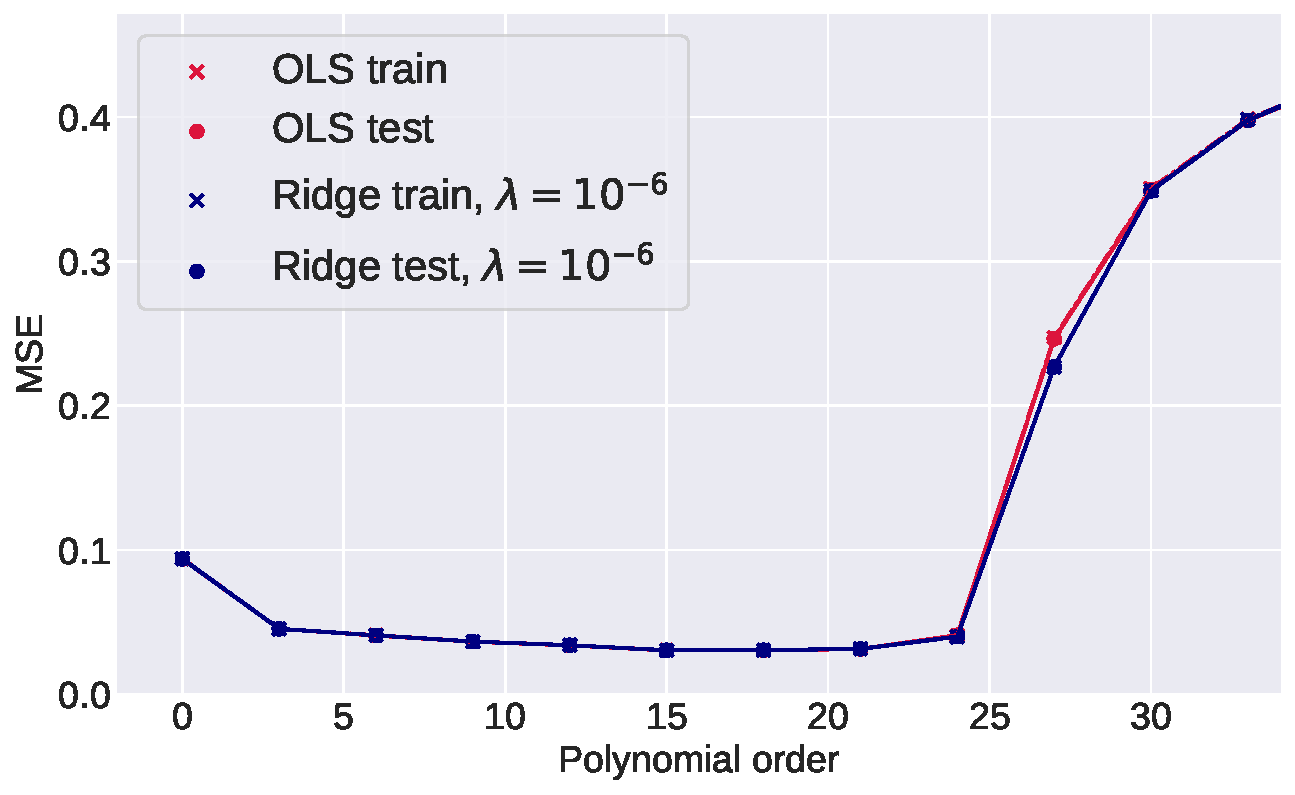
\includegraphics[scale=0.4]{../figs/OLS_Ridge_0to2divergence.pdf}
    \caption{Plot illustrating the same setup as \cref{fig:Terrain_8x8_poly100}, except explanatory variables are shifted to $x,y\in [0,\, 2]$. This causes the MSE to diverge at around polynomial order 25.}
    \label{fig:0to2divergence}
\end{figure}



Another indication of the numerical instability can be seen from looking at the condition number (discussed in \cref{subsec:singularity}) of the design matrix, and the Hessian matrix (which is the one we are actually inverting). In \cref{fig:cond_num} the condition number of both matrices are plotted, showing the large numerical instability of higher order models.

An interesting correlation is that the conditioning number for $\lambda = 10^{-6}$ stops increasing exactly at the same point (order ~25) that OLS starts outperforming Ridge, as we saw in figure \cref{fig:Terrain_8x8_poly100}. Apperantly, from order ~25 and onward, the $\lambda$ value dominates the size of the columns, causing further columns to add less to the predicitive capabilities, but also produce less numerical instability.

\begin{figure}[h!]
    \centering
    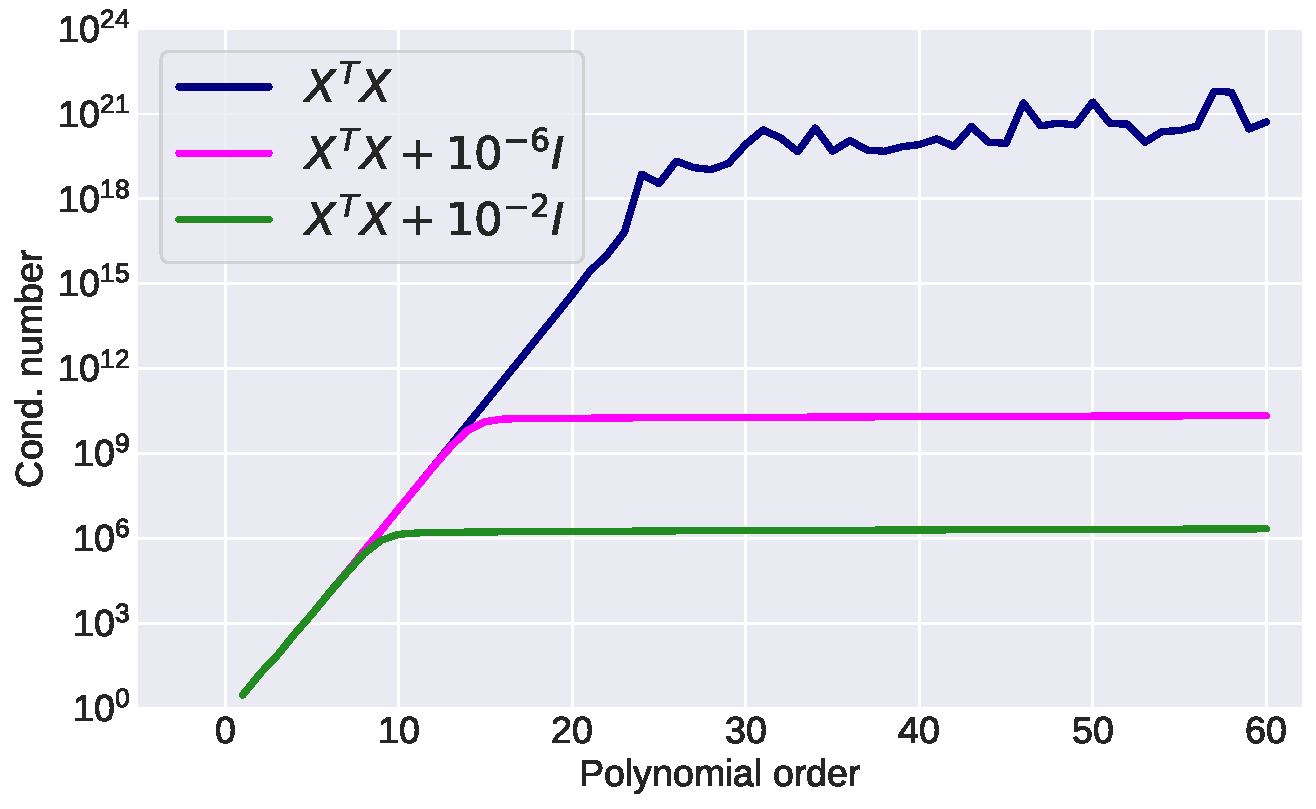
\includegraphics[scale=0.4]{../figs/cond.pdf}
    \caption{Plot showing the condition number of the matrix $\vb{A}=\vb{X^T}\vb{X}$ as function of polynomial order. $\vb{A}$ for Ridge, with $\lambda$ of $10^{-2}$ and $10^{-6}$ is also shown. The condition number, and thereby numerical instability, grows large for large polynomial orders, but stabilizes around $10^{20}$. The lambdas have a clear suppression effect on the condition number, stabilizing the condition number much earlier.}
    \label{fig:cond_num}
\end{figure}



Figure \cref{fig:cond_num2} shows the same conditioning plot, but for the explanatory variables in the interval $[0,\, 2]$, just as we looked at in \cref{fig:0to2divergence}. Here the reason for the diverging behavior becomes even more obvious. The conditioning number of the Hessian matrix not only increases a lot quicker (it is ~$10^{16}$ at poly order 10, to the $~10^{7}$ in the former case), but it also never stops diverging. Adding a $\lambda$ term now also have virtually no effect, which explains why Ridge also diverges in a similar fashion to OLS.

\begin{figure}[h!]
    \centering
    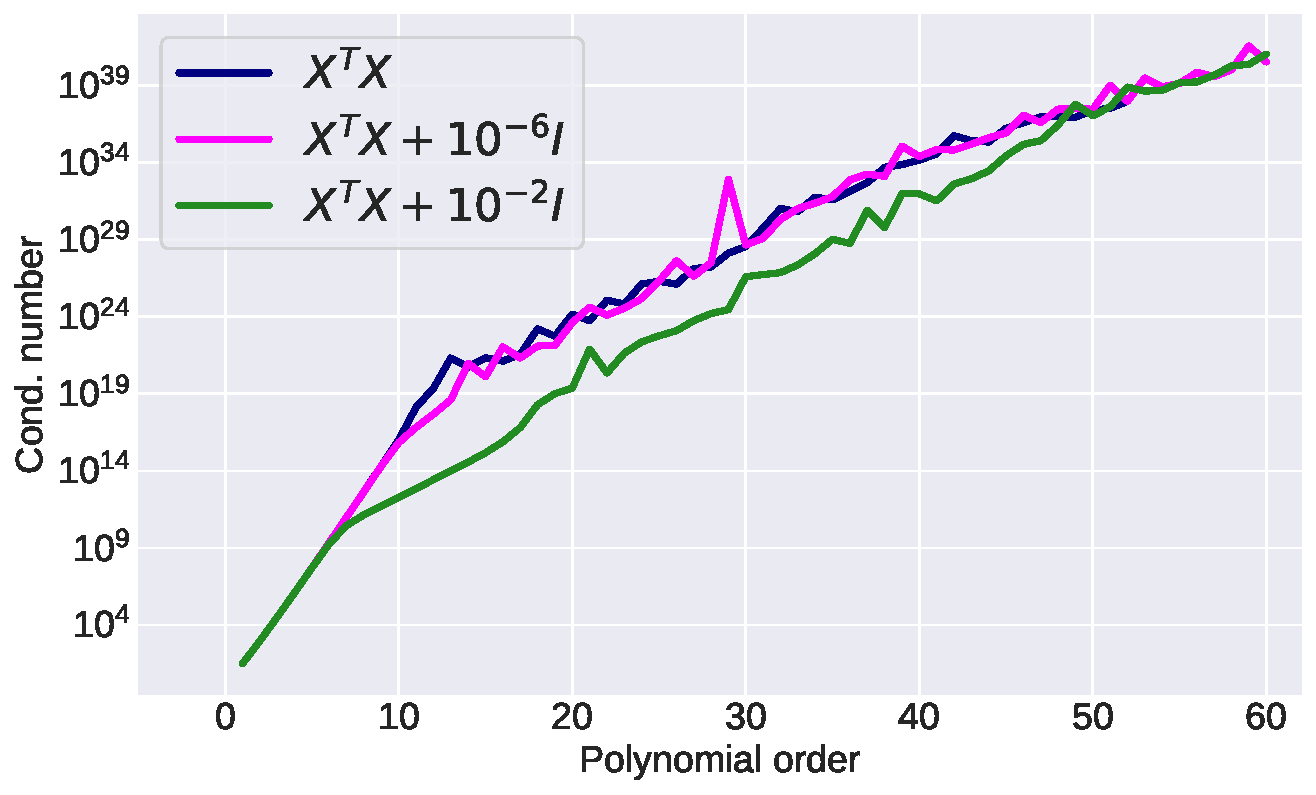
\includegraphics[scale=0.4]{../figs/cond_02.pdf}
    \caption{Figure with same setup as \cref{fig:cond_num}, except explanatory variables are shifted to $x,y \in [0,\, 2]$. The condition number now never stops increasing, and the lambdas no longer have the same suppression effect.}
    \label{fig:cond_num2}
\end{figure}


We are able to provoke overfitting without running into the aforementioned problems by reducing the number of datapoints. Downsampling the image by 32x32, we see from \cref{fig:overfit32} that the testing error of OLS increases from its lowest point around order 25. From there, the error diverges very rapidly, especially from order 45 and higher. This overfit increases much more rapidly than it did for the Franke data, which was more gradual. A good theory as to why is that, downsampled by 32x32, the image contains only 112x56 pixels. The error diverges when the polynomial order starts approaching the number of points on the shortest axis. We know that a polynomial of degree $N$ is capable of perfectly fitting a dataset of $N$ points. This allows for a massive overfitting along the x-axis.

Ridge is a lot more resistant, but we see a slight increase in higher orders, which we didn't see for the less downsampled image.

\begin{figure}[h!]
    \centering
    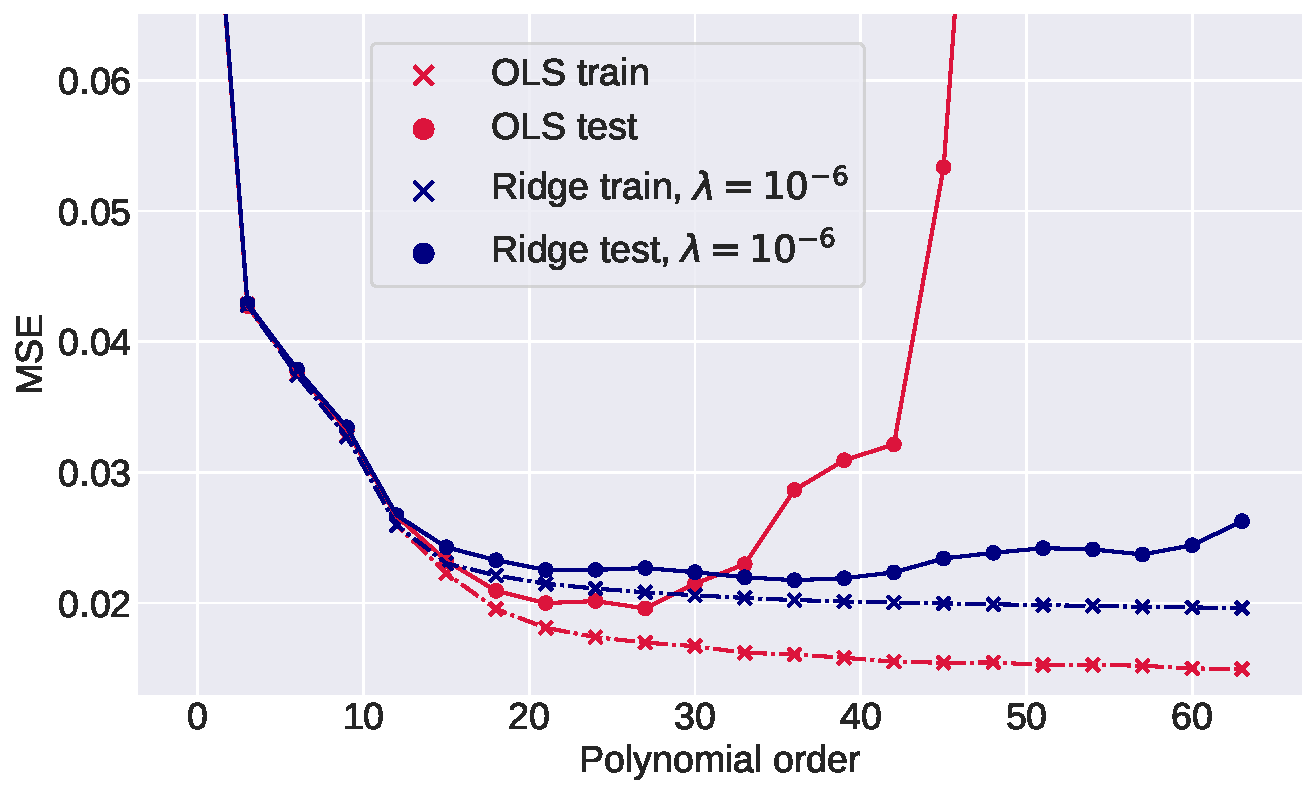
\includegraphics[scale=0.4]{../figs/OLS_Ridge_Terrain_32sample.pdf}
    \caption{Plot showing the same setup as \cref{fig:Terrain_8x8_poly100}, except image is downsampled by 32x32. OLS heavily overfits for polynomial orders above 30. Ridge seems almost uneffected by the increased complexity, holding a relatively steady training MSE.}
    \label{fig:overfit32}
\end{figure}


\subsubsection{Terrain Data Bootstrap}
In \cref{fig:Bootstrap_terrain_ols}, we see the results of preforming our bias-variance split, using bootstrapping, on the 32x32 downsampled Terrain data. This downsampling was selected because we were unable to provoke overfitting on less downsampled data. We see a very similar trend as we did when applying the bootstrap to the Franke data, where the bias falls together with the total error, down to some level, before they both increase again. This increase seem to come together with the sudden increase in variance. Again, while we in theory expected the raise in total error to come solely from an increase in variance, there is also a contribution from an increase in bias, which is not understood. The equivalent results for Ridge and Lasso are found in the appendix \ref{asec:Bias_Var_results}. 

\begin{figure}[h!]
    \centering
    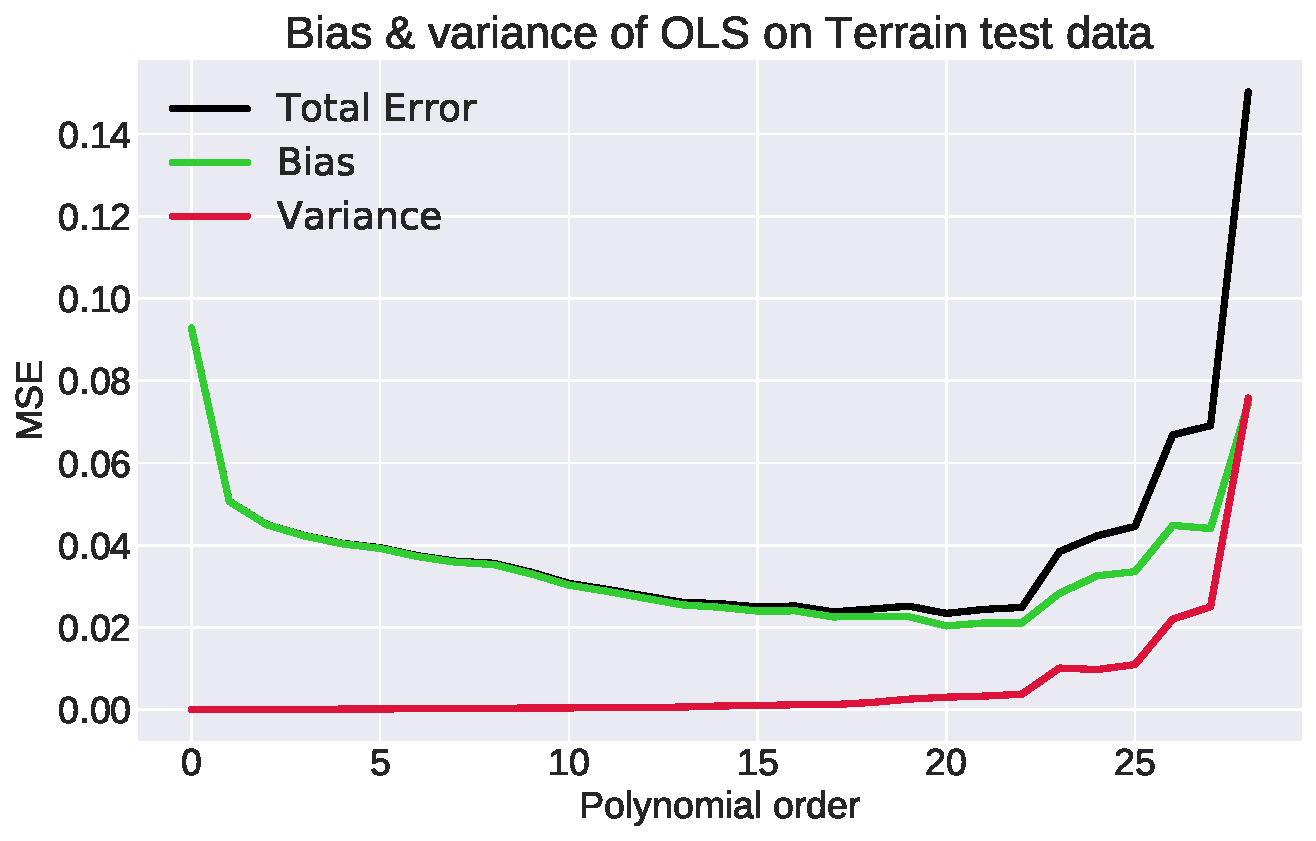
\includegraphics[scale=0.4]{../figs/BV_bootstrap_Terrain_OLS.pdf}
    \caption{Plot showing the bias variance tradeoff as a function of polynomial order on the terrain test set. Like for the Franke data in \cref{fig:Boostrap_franke_ols} we can see how the bias is prominent at low complexity, while for higher complexity the variance of the model increase. Here too the bias start increasing for higher complexity which is unexpected.}
    \label{fig:Bootstrap_terrain_ols}
\end{figure}



\subsection{Best Fit Terrain}
Having studied the implications of both the model complexity and hyperparamters, we can safely conclude that, as long as we're dealing with a large amount of data, OLS with a high order polynomial gives the best fit. We therefore employ a 80 degree polynomial on the terrain data, downsampled only by 4x4. In \cref{fig:BestFitTerrain} we see the result, together with an absolute difference plot. We see that the fit does a good job at capturing the large scale structures of the data, while struggling with the finer details. The final fit results can be seen in \cref{tab:error_metrics_terrain_data_higherorder}.

\begin{table}[h!]
\centering
\begin{tabular}{l|l|l|}
\cline{2-3}
                                            & \textbf{MSE} & \textbf{R2} \\ \hline
\multicolumn{1}{|l|}{\textbf{Terrain data}} & 0.018        & 0.761       \\ \hline
\end{tabular}
\caption{Table showing the error metrics when fitting the terrain data using OLS regression with polynomial of order 80.}
\label{tab:error_metrics_terrain_data_higherorder}
\end{table}

\begin{figure}[h!]
    \centering
    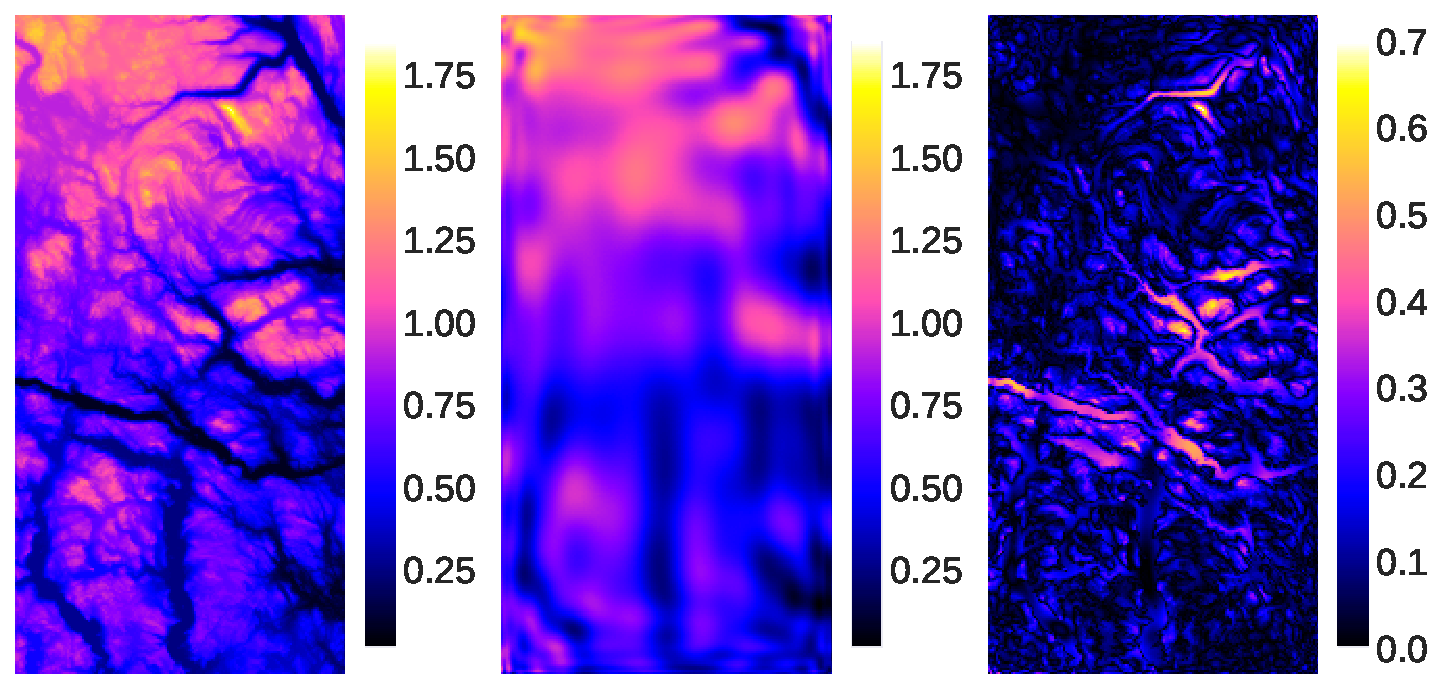
\includegraphics[scale=0.4]{../figs/BestFitTerrain.pdf}
    \caption{Left: Original terrain image, downsampled by 4x4. Center: Best fit OLS, polynomial order 80, with K fold validation. Right: Absolute difference between the former two. We clearly see that the fit retains the larger trends of the image, but struggles to capture the more fine-structured qualities.}
    \label{fig:BestFitTerrain}
\end{figure}


\section{Conclusion}
The goal of this project was to explore the properties, advantages, and behavior of three methods of linear regression - OLS, Ridge, and Lasso regression, especially in the context of bias-variance tradeoff and over/underfitting. We also wanted to put the methods into the context of common machine learning techniques, like cross validation and resampling. For this, two datasets were applied, a generic dataset, generated from Franke's function with added noise, and a real Terrain map.

We found that, for some optimal complexity (translating to polynomial degree in our model), OLS outperformed both Ridge and Lasso for both datasets. This optimal polynomial order was found to be around 5 for the Franke data, and arbitrarily high for Terrain data, due to numerical limitations. OLS achieved a MSE of 0.004 and and R2 score of 0.820 against the noiseless Franke data (while trained on the noisy data) using a 5th order polynomial, and a MSE of 0.018 and a R2 score of 0.761 on the Terrain data, using a 80th order polynomial.

While OLS performed best under ideal circumstances, we found that Ridge, and especially Lasso, was a lot more resistant to overfitting than OLS. For only slightly higher complexities than ideal, Lasso and Ridge vastly outperformed OLS. Ridge had some tendency to overfit, while Lasso usually had none. Lasso was, however, unable to run in reasonable time for larger systems, as its implicit solutions leaves it costly to solve.

We also found strong numeric instabilities in the design matrix, which was found to have very high conditioning numbers, of the order $10^{20}~10^{40}$ for moderately complex systems. This raised doubts about the validity of the results for higher order fits, where higher order columns of the design matrix is suppressed.

The presence of overfitting was also found to strongly correlate with the size of the dataset we performed our regression on. We found it necessary to downsample our dataset in order to provoke overfitting at all, because the numerical instabilities gave suppression effects before a high enough complexity level could be reached.

\section{Future Work}
We found the chosen datasets to be less than ideal for demonstrating the various properties of the regression methods. The datasets have explanatory variables (orders of the x and y axis) which are hard to intuitively interpret, and there is no specific reason why one should thing that a polynomial is a good way of fitting a terrain. We would like to perform the same analysis on a dataset where the correlation between input and output variables can be more intuitively understood.

We would also like to study in larger detail the numerical problems we ran into. It was clear to us that, for moderate complexities and higher, numerics were starting to play a role in our results, caused by ill-conditioned design matrices. We would like to further explore how this affected our results, and perhaps look for ways to circumvent them.







%\end{multicols}
\onecolumn
\bibliography{ref}
\newpage
\begin{appendices}
\section{Bias-Variance derivation}
\label{asec:Bias-Variance-derivation}
In this section we will show the derivation of \cref{eq:Bias_variance_tradeoff}. We start by the definition of mean squared error, \cref{eq:MSE}. This is manipulated by adding and subtracting the expectation value of our fit inside the expression. By doing this we can order the equation in a way that decompose the MSE in to two contributions; the bias and the variance. In this derivation the following notation is used;
\begin{itemize}
    \item The data is expressed as $\bm{y} = \bm{f} + \bm{\epsilon}$, where $\bm{f}$ is deterministic and $\bm{\epsilon}$ is stochastic noise from the normal distribution $\bm{\epsilon} \sim N(0,\sigma^2)$. This means that $\forv{\bm{f}} = \bm{f}$, $\forv{\bm{\epsilon}} = 0$, $\mathrm{Var}(\bm{\epsilon}) = \forv{\bm{\epsilon}^2} = \sigma^2$
    \item The fit is expressed as $\bm{\tilde{y}} = \bm{X}\bm{\beta}$
\end{itemize}
\begin{align*}
    \forvsum{(y_i - \tilde{y}_i)^2} &= \forv{(\bm{y} - \bmt{y})^2} = \forv{(\bm{f} + \bm{\epsilon} - \bmt{y} + \forv{\bmt{y}} - \forv{\bmt{y}})^2}
    \\
    \qq*{expanding the parenthesis:}
    \\
    \forv{
        (\bm{f} + \bm{\epsilon} - \bmt{y} + \forv{\bmt{y}} - \forv{\bmt{y}})^2} &=
        \forv{
        \begin{aligned}
        &\bm{f}^2 - 2 \bm{f}\forv{\bmt{y}}+\forv{\bmt{y}}^2
        \\
        &+ \bmt{y}^2 - 2 \bmt{y}\forv{\bmt{y}} + \forv{\bmt{y}}^2
        \\
        & + \bm{\epsilon}^2 + \bm{\epsilon} \left(2\bm{f} + \bmt{y} - \bmt{y} + 2\left(\forv{\bmt{y}} -\forv{\bmt{y}}\right)^{\vphantom{2}} \right)
        \\
        & + 2\left(\bm{f}\forv{\bmt{y}}- \bm{f}\bmt{y} + \bmt{y}\forv{\bmt{y}} - \forv{\bmt{y}}^2\right)
        \end{aligned}
    }
    \\
    \qq*{using} \forv{\bm{\epsilon}} = 0\text{:}
    \\
    &= \forv{
        \begin{aligned}
        &\left(\bm{f}-\forv{\bmt{y}}\right)^2 + \left(\bmt{y}-\forv{\bmt{y}}\right)^2 + \bm{\epsilon}^2
        \\
        & + 2 \left(\bm{f}\forv{\bmt{y}} - \bm{f}\bmt{y} + \bmt{y}\forv{\bmt{y}} - \forv{\bmt{y}}^2\right)
        \end{aligned}
        }
    \\
    \qq*{\text{$\mathbb{E}[x]$} is a linear operator:}
    \\
    &=
        \forv{\left(\bm{f}-\forv{\bmt{y}}\right)^2} +         \forv{\left(\bmt{y}-\forv{\bmt{y}}\right)^2} +         \forv{\bm{\epsilon}^2} 
        \\
        &\quad + 2 \forv{\left(\bm{f}\forv{\bmt{y}} - \bm{f}\bmt{y} +  \bmt{y}\forv{\bmt{y}} - \forv{\bmt{y}}^2\right)}
\end{align*}
Now we have separated out the three terms we want, so for this to be equal the expression in \cref{eq:Bias_variance_tradeoff}, the last term must be equal to zero. To show this we factor out the deterministic terms out of the expectation value.
\begin{align*}
    \forv{\left(\bm{f}\forv{\bmt{y}} - \bm{f}\bmt{y} +  \bmt{y}\forv{\bmt{y}} - \forv{\bmt{y}}^2\right)}
    &=
    \forv{\left(\forv{\bmt{y}}-\bmt{y}\right)\left(\bm{f}-\forv{\bmt{y}}\right)^{\vphantom{2}}}
    \\
    &=
    \left(\bm{f}-\forv{\bmt{y}}\right)\forv{\bmt{y}-\forv{\bmt{y}}^{\vphantom{2}}}
    \\
    &=
    \left(\bm{f}-\forv{\bmt{y}}\right)\left(\forv{\bmt{y}}-\forv{\forv{{\bmt{y}}}}^{\vphantom{2}}\right)
    \\
    \qq*{where}\forv{\forv{\bmt{y}}} = \forv{\bmt{y}}
    \\
    &= 0
\end{align*}
So the MSE can be expressed, inserting the summation form of the expectation value
\begin{align*}
    \text{MSE}\left(\bm{y},\bmt{y}\right) &=    \forv{\left(\bm{f}-\forv{\bmt{y}}\right)^2} +         \forv{\left(\bmt{y}-\forv{\bmt{y}}\right)^2} + \sigma^2
    \\
    &= \forvsum{\left(\bm{f}-\forv{\bmt{y}}\right)^2} + \forvsum{\left(\bmt{y}-\forv{\bmt{y}}\right)^2} + \sigma^2
\end{align*}

\newpage
\section{Additional Bias-Variance Results}
\label{asec:Bias_Var_results}
Here we present additional results from our bias variance tradeoff experiments which we chose to not to include with the rest of the results to reduce cluttering. As discussed for the results from OLS, the bias is high for low complexity which leads to a high MSE. Increasing complexity reduces the bias which leads to an optimal polynomial order. In the case of OLS we could see how the variance started to increase when the model started overfitting, but using Ridge and Lasso we are not able to run calculations with high enough polynomial order to make this trend evident, at least not for the terrain data where the MSE and the bias is almost equal. For the Franke data we see how the variance start to increasing ever so slightly for higher complexity, and still the bias is also increasing which is unexpected.

\begin{figure}[h!]
    \begin{subfigure}[t]{0.45\textwidth}
    \centering
    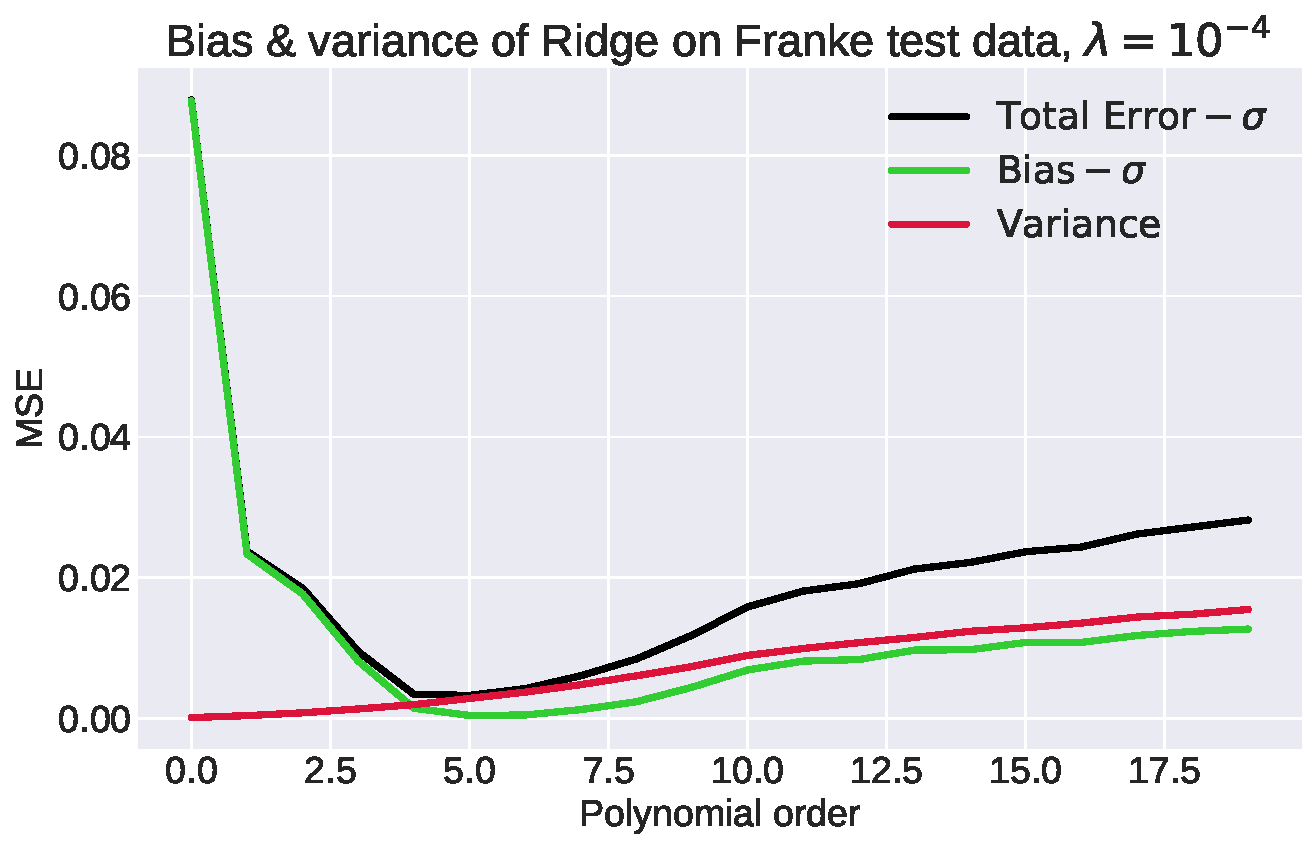
\includegraphics[scale=0.4]{../figs/BV_bootstrap_Franke_Ridge.pdf}
    \caption{}
    \label{fig:boostrap_franke_ridge}
    \end{subfigure}
    %
    \begin{subfigure}[t]{0.45\textwidth}
    \centering
    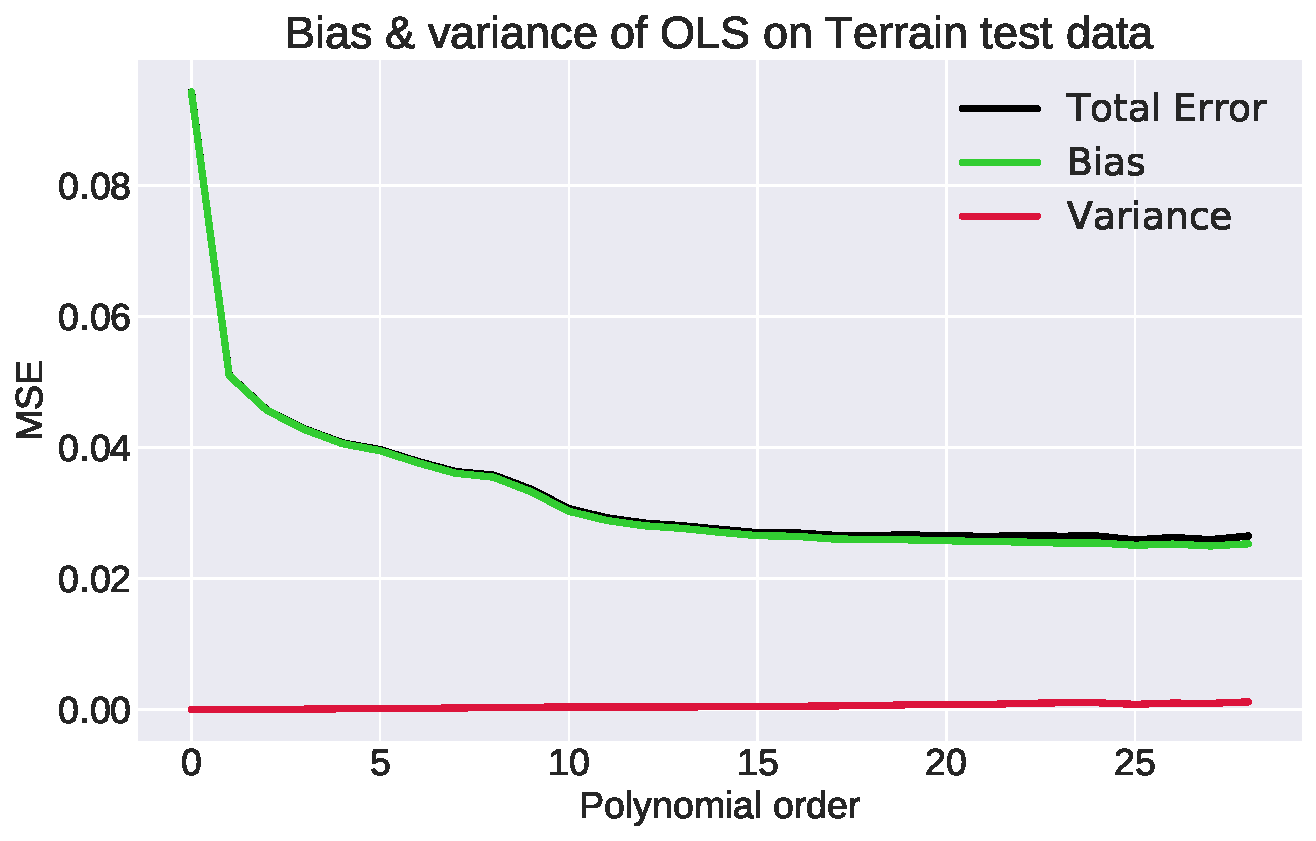
\includegraphics[scale=0.4]{../figs/BV_bootstrap_Terrain_Ridge.pdf}
    \caption{}
    \label{fig:boostrap_terrain_ridge}
    \end{subfigure}
    %
    \centering
    \begin{subfigure}[t]{0.45\textwidth}
    \centering
    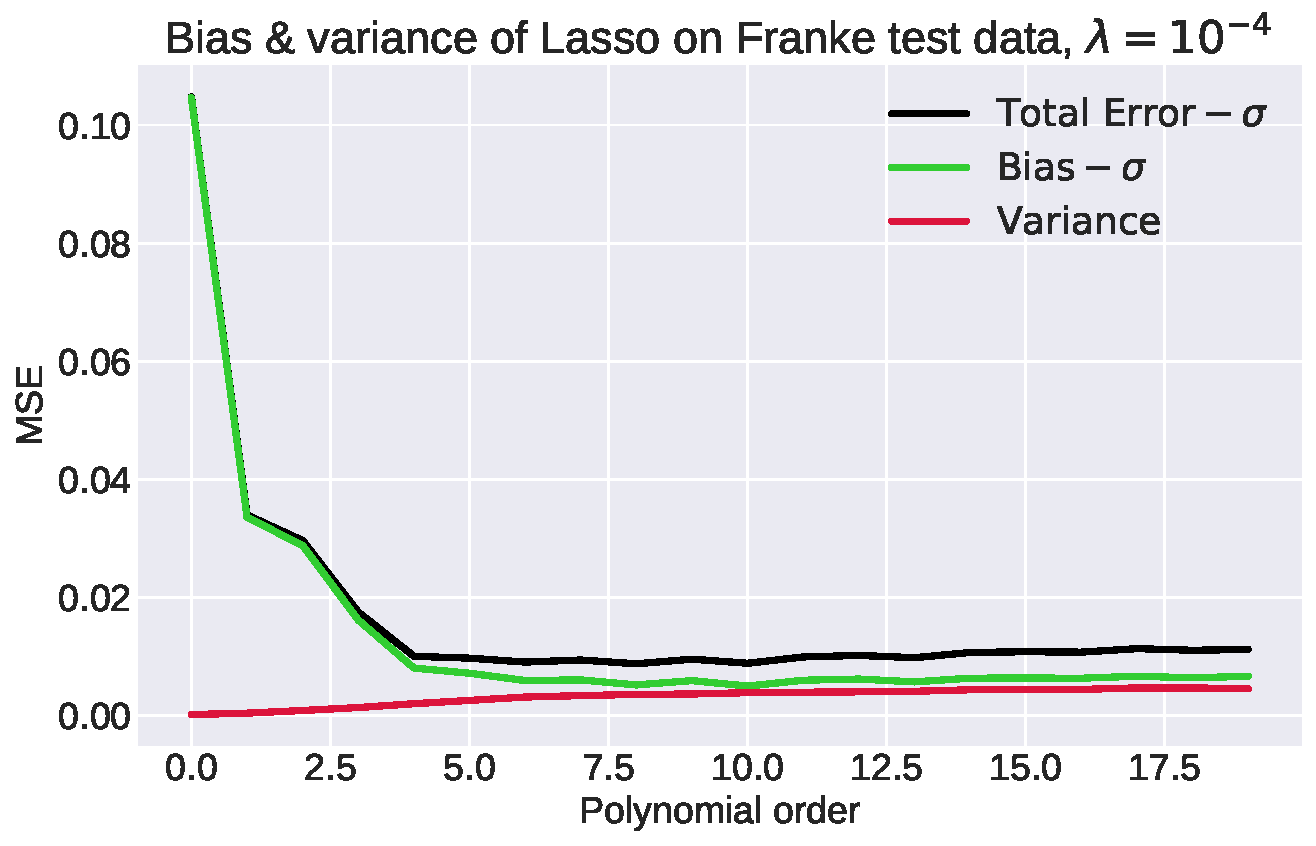
\includegraphics[scale=0.4]{../figs/BV_bootstrap_Franke_Lasso.pdf}
    \caption{}
    \label{fig:boostrap_franke_lasse}
    \end{subfigure}
    %
    \begin{subfigure}[t]{0.45\textwidth}
    \centering
    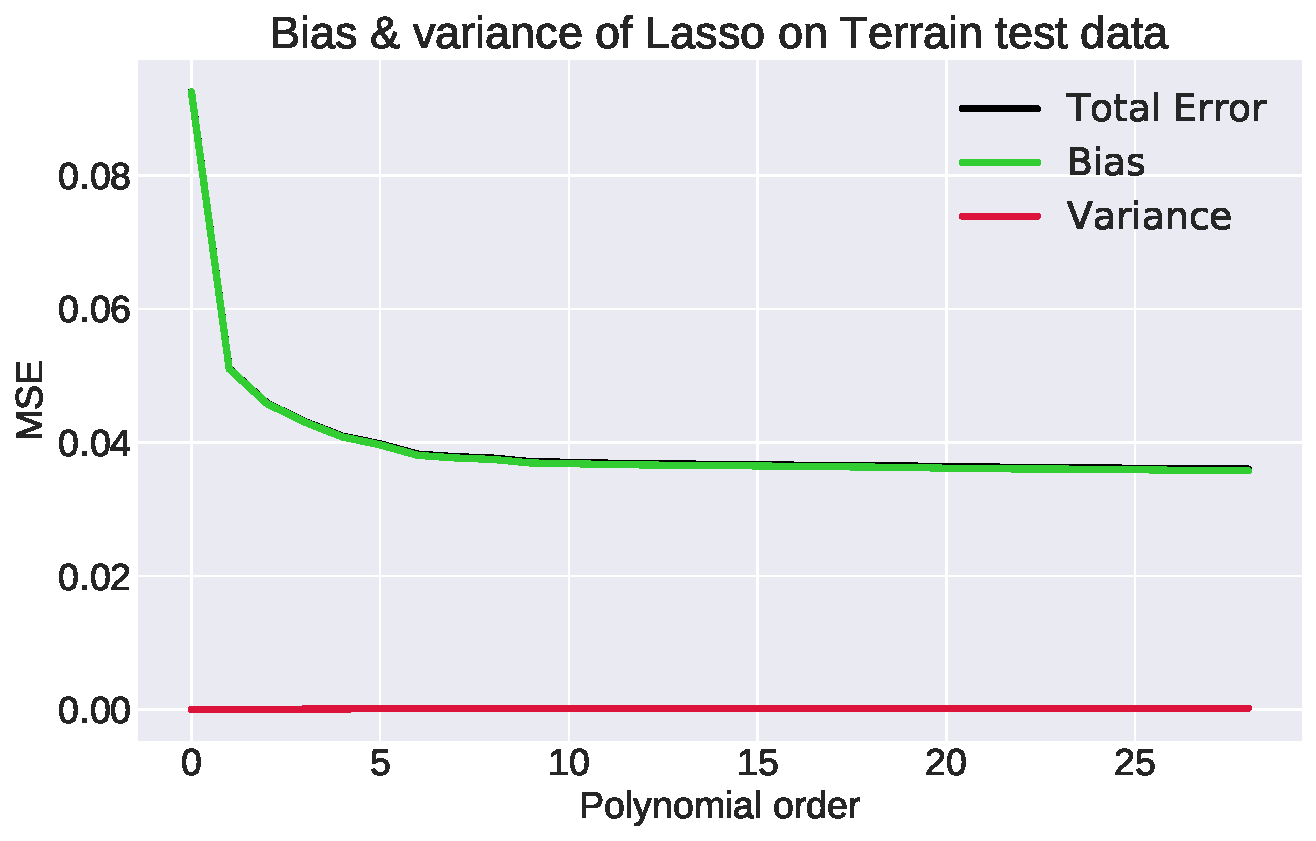
\includegraphics[scale=0.4]{../figs/BV_bootstrap_Terrain_Lasso.pdf}
    \caption{}
    \label{fig:boostrap_terrain_lasso}
    \end{subfigure}
    %
\caption{Bias-variance results for Ridge in (a) and (b), Lasso in (c) and (d), all run with $\lambda = 10^{-4}$. For the Franke data the irreducible error is subtracted from the bias and the MSE.}
\end{figure}

\end{appendices}
\end{document}
